\documentclass[12pt,]{article}
\usepackage{lmodern}
\usepackage{amssymb,amsmath}
\usepackage{ifxetex,ifluatex}
\usepackage{fixltx2e} % provides \textsubscript
\ifnum 0\ifxetex 1\fi\ifluatex 1\fi=0 % if pdftex
  \usepackage[T1]{fontenc}
  \usepackage[utf8]{inputenc}
\else % if luatex or xelatex
  \ifxetex
    \usepackage{mathspec}
  \else
    \usepackage{fontspec}
  \fi
  \defaultfontfeatures{Ligatures=TeX,Scale=MatchLowercase}
    \setmainfont[]{Times New Roman}
\fi
% use upquote if available, for straight quotes in verbatim environments
\IfFileExists{upquote.sty}{\usepackage{upquote}}{}
% use microtype if available
\IfFileExists{microtype.sty}{%
\usepackage{microtype}
\UseMicrotypeSet[protrusion]{basicmath} % disable protrusion for tt fonts
}{}
\usepackage[margin=2.54cm]{geometry}
\usepackage{hyperref}
\hypersetup{unicode=true,
            pdftitle={Examining the Hydrologic Properties of the Missouri River Basin},
            pdfauthor={Rachel Bash, Keqi He, Caroline Watson, and Haoyu Zhang},
            pdfborder={0 0 0},
            breaklinks=true}
\urlstyle{same}  % don't use monospace font for urls
\usepackage{color}
\usepackage{fancyvrb}
\newcommand{\VerbBar}{|}
\newcommand{\VERB}{\Verb[commandchars=\\\{\}]}
\DefineVerbatimEnvironment{Highlighting}{Verbatim}{commandchars=\\\{\}}
% Add ',fontsize=\small' for more characters per line
\usepackage{framed}
\definecolor{shadecolor}{RGB}{248,248,248}
\newenvironment{Shaded}{\begin{snugshade}}{\end{snugshade}}
\newcommand{\AlertTok}[1]{\textcolor[rgb]{0.94,0.16,0.16}{#1}}
\newcommand{\AnnotationTok}[1]{\textcolor[rgb]{0.56,0.35,0.01}{\textbf{\textit{#1}}}}
\newcommand{\AttributeTok}[1]{\textcolor[rgb]{0.77,0.63,0.00}{#1}}
\newcommand{\BaseNTok}[1]{\textcolor[rgb]{0.00,0.00,0.81}{#1}}
\newcommand{\BuiltInTok}[1]{#1}
\newcommand{\CharTok}[1]{\textcolor[rgb]{0.31,0.60,0.02}{#1}}
\newcommand{\CommentTok}[1]{\textcolor[rgb]{0.56,0.35,0.01}{\textit{#1}}}
\newcommand{\CommentVarTok}[1]{\textcolor[rgb]{0.56,0.35,0.01}{\textbf{\textit{#1}}}}
\newcommand{\ConstantTok}[1]{\textcolor[rgb]{0.00,0.00,0.00}{#1}}
\newcommand{\ControlFlowTok}[1]{\textcolor[rgb]{0.13,0.29,0.53}{\textbf{#1}}}
\newcommand{\DataTypeTok}[1]{\textcolor[rgb]{0.13,0.29,0.53}{#1}}
\newcommand{\DecValTok}[1]{\textcolor[rgb]{0.00,0.00,0.81}{#1}}
\newcommand{\DocumentationTok}[1]{\textcolor[rgb]{0.56,0.35,0.01}{\textbf{\textit{#1}}}}
\newcommand{\ErrorTok}[1]{\textcolor[rgb]{0.64,0.00,0.00}{\textbf{#1}}}
\newcommand{\ExtensionTok}[1]{#1}
\newcommand{\FloatTok}[1]{\textcolor[rgb]{0.00,0.00,0.81}{#1}}
\newcommand{\FunctionTok}[1]{\textcolor[rgb]{0.00,0.00,0.00}{#1}}
\newcommand{\ImportTok}[1]{#1}
\newcommand{\InformationTok}[1]{\textcolor[rgb]{0.56,0.35,0.01}{\textbf{\textit{#1}}}}
\newcommand{\KeywordTok}[1]{\textcolor[rgb]{0.13,0.29,0.53}{\textbf{#1}}}
\newcommand{\NormalTok}[1]{#1}
\newcommand{\OperatorTok}[1]{\textcolor[rgb]{0.81,0.36,0.00}{\textbf{#1}}}
\newcommand{\OtherTok}[1]{\textcolor[rgb]{0.56,0.35,0.01}{#1}}
\newcommand{\PreprocessorTok}[1]{\textcolor[rgb]{0.56,0.35,0.01}{\textit{#1}}}
\newcommand{\RegionMarkerTok}[1]{#1}
\newcommand{\SpecialCharTok}[1]{\textcolor[rgb]{0.00,0.00,0.00}{#1}}
\newcommand{\SpecialStringTok}[1]{\textcolor[rgb]{0.31,0.60,0.02}{#1}}
\newcommand{\StringTok}[1]{\textcolor[rgb]{0.31,0.60,0.02}{#1}}
\newcommand{\VariableTok}[1]{\textcolor[rgb]{0.00,0.00,0.00}{#1}}
\newcommand{\VerbatimStringTok}[1]{\textcolor[rgb]{0.31,0.60,0.02}{#1}}
\newcommand{\WarningTok}[1]{\textcolor[rgb]{0.56,0.35,0.01}{\textbf{\textit{#1}}}}
\usepackage{graphicx,grffile}
\makeatletter
\def\maxwidth{\ifdim\Gin@nat@width>\linewidth\linewidth\else\Gin@nat@width\fi}
\def\maxheight{\ifdim\Gin@nat@height>\textheight\textheight\else\Gin@nat@height\fi}
\makeatother
% Scale images if necessary, so that they will not overflow the page
% margins by default, and it is still possible to overwrite the defaults
% using explicit options in \includegraphics[width, height, ...]{}
\setkeys{Gin}{width=\maxwidth,height=\maxheight,keepaspectratio}
\IfFileExists{parskip.sty}{%
\usepackage{parskip}
}{% else
\setlength{\parindent}{0pt}
\setlength{\parskip}{6pt plus 2pt minus 1pt}
}
\setlength{\emergencystretch}{3em}  % prevent overfull lines
\providecommand{\tightlist}{%
  \setlength{\itemsep}{0pt}\setlength{\parskip}{0pt}}
\setcounter{secnumdepth}{5}
% Redefines (sub)paragraphs to behave more like sections
\ifx\paragraph\undefined\else
\let\oldparagraph\paragraph
\renewcommand{\paragraph}[1]{\oldparagraph{#1}\mbox{}}
\fi
\ifx\subparagraph\undefined\else
\let\oldsubparagraph\subparagraph
\renewcommand{\subparagraph}[1]{\oldsubparagraph{#1}\mbox{}}
\fi

%%% Use protect on footnotes to avoid problems with footnotes in titles
\let\rmarkdownfootnote\footnote%
\def\footnote{\protect\rmarkdownfootnote}

%%% Change title format to be more compact
\usepackage{titling}

% Create subtitle command for use in maketitle
\providecommand{\subtitle}[1]{
  \posttitle{
    \begin{center}\large#1\end{center}
    }
}

\setlength{\droptitle}{-2em}

  \title{Examining the Hydrologic Properties of the Missouri River Basin}
    \pretitle{\vspace{\droptitle}\centering\huge}
  \posttitle{\par}
  \subtitle{\url{https://github.com/cwatson1013/Hydrologic_Data_Analysis_Final_Proj}}
  \author{Rachel Bash, Keqi He, Caroline Watson, and Haoyu Zhang}
    \preauthor{\centering\large\emph}
  \postauthor{\par}
    \date{}
    \predate{}\postdate{}
  
\usepackage{booktabs}
\usepackage{longtable}
\usepackage{array}
\usepackage{multirow}
\usepackage{wrapfig}
\usepackage{float}
\usepackage{colortbl}
\usepackage{pdflscape}
\usepackage{tabu}
\usepackage{threeparttable}
\usepackage{threeparttablex}
\usepackage[normalem]{ulem}
\usepackage{makecell}
\usepackage{xcolor}

\begin{document}
\maketitle
\begin{abstract}
The Missouri River provides critical water resources that drives the
region's agriculture, industry, and ecosystems. This is a region that
experiences surface water variability, characterized by damaging floods
and severe droughts, greatly impacting the agricultural production of
the area. It is reported that a serious flood disaster occurred in the
lower Missouri River in the spring of 2019 and the Missouri River
experienced severe drought in 2012-2013. This project highlights the
changes in stream flow and water quality over time, and identifies key
characteristics of the river. Twenty two sites across the lower Missouri
River Basin were examined in order to get a fuller picture of the
Missouri River and its tributaries over time. By analyzing the trend of
the Missouri River discharge, we can predict future changes in the
Missouri River flow to provide a reference for water resources
management. In addition, we focus on the stream flow and water quality
of Missouri River during March to July, 2019 to see how discharge
influence the water quality and what can be done to keep the water in
the Missouri River in good quality.
\end{abstract}

\newpage
\tableofcontents 
\newpage
\listoftables 
\newpage
\listoffigures 
\newpage

\hypertarget{research-question-and-rationale}{%
\section{Research Question and
Rationale}\label{research-question-and-rationale}}

The Missouri River is the largest river in North America (2,540 miles)
and has the second largest watershed (529,000 mi\textsuperscript{2}/339
acres, U.S.-Canada). Its watershed covers portions of ten states, which
account for approximately one-sixth of the continental United States, as
well as a small part of Canada. The headwater is located in the
Bitterroot Mountains River of northwestern Wyoming and southwestern
Montana. The watershed is home to around 12 million people in 1990, and
has been inhabited by indigenous people for millennia. Demands for
managing the river for the benefit of human livelihood has resulted in
drastic modification in the river and the floodplains. Numerous
reservoirs and dams have been constructed, of which six major dams were
built on the mainstream, following the Pick-Sloan Plan in 1944. Now, the
river is used intensively in multiple ways, including municipal,
agricultural, hydropower, recreation, flood control etc.

Within the 328 million acres of the basin's total area in the United
States, 95\% is related to agricultural uses, while the rest dedicated
for recreation, fish and wildlife, and urban. More than half of the
total is pasture and range grassland primarily for grazing, and cropland
consists of almost 104 million acres, which is 32\% of the whole basin.
Irrigated land comprises 7.4 million acres, and 6.9 million acres are
intensively cropped. Water bodies, on the other hand, cover 3.9 million
acres. In spite of the low proportion of water areas (1.2\%), they are
the pivotal foundation for agricultural or other usages, and thus
critical to the whole region's economy.

Along with the agricultural, urban, and industrial development in the
region is nutrient loading and enrichment in water bodies, especially
for nitrogen (N) and phosphorus (P). Unlike other regions, agricultural
input through fertilizer is the predominant anthropogenic source for
nutrient in water bodies in the whole basin. Regardless of the major
anthropogenic source, nutrient enrichment is considered nationally as
one of the leading factors for water quality impairment. According to
USEPA 303(d) lists, more than 160 stream reaches, lakes, or reservoirs
were reported by USEPA to be nutrient-related impaired in 2006.

In addition to change in nutrient concentration, discharge appears to be
highly variable in the basin, and both severe drought and flooding
events occurred in the basin in the past. For example, in the spring and
summer of 2011, an unprecedented flooding event caused over \$2 billion
damage FEMA disaster declaration was made in all states along the
Missouri River. Subsequently, in 2012, a drought even struck the Central
Great Plain, including the basin, and inflicted at least \$12 billion of
loss before July, 2012. Recently, another flooding event occurred in the
spring of 2019.

Given all the background information above, we would like to know the
current state of Missouri River and its tributaries, with a focus on the
changing pattern in discharge and nutrient. We are interested in how the
dramatic change in discharge (i.e.~water quantity) could potentially
interact with nutrient enrichment (i.e.~water quality). Also, we
examined a few specific flooding events, during which changes in both
water quality and quantity were well recorded, so that we could make
concrete inference on the interplay between quantity and quality.
Finally, based on the pattern in the past and the best model we could
fit, we attempted to predict the likely future conditions and trends in
the Missouri River Basin.

\newpage

\hypertarget{dataset-information}{%
\section{Dataset Information}\label{dataset-information}}

The data we are analyzing comes from the United States Geological Survey
(USGS) database called the National Water Information System interface,
or NWIS. We pulled data from the interface using the R package
\texttt{dataRetrieval}. Because we are interested in the lower Missouri
River basin, we pulled sites from each HUC4 subbasin from 1020 to 1030
(see Figure below). We chose these subbasins because they had a variety
of tributaries that all flowed into the Missouri River, and we wanted a
variety of river sizes and lengths. We filtered these subbasin queries
to only show us sites that had discharge, nitrogen, and phosphorus data.
Once we found the sites with all of this data, we chose 2 sites from
each HUC sub basin as our 22 ``best sites''. Our best sites had the
overall best time period range for all of our ``must have'' variables.
We retrieved data on water quantity, water quality (N, P
concentrations), pH, and coliform concentrations. @ref\{tab:table\}
illustrates the variables we examined and the number of sites in our
area of interest that had quality data for each.

Only seven sites within our HUC subbasin boundary contained any high
frequency discharge and nitrogen data. Therefore, we also looked at
these 7 sites in order to do analyses and answer our research question
about flooding.

After doing initial data wrangling and analysis on our 22 ``best
sites'', we decided to pare it down further and only do subsequent
analyses on \textbf{10} sites. While we initially wanted to look at many
sites that were varied in size and location, we determined that it was
too many to look at and draw relevant conclusions from.

We have three main datasets:

\begin{itemize}
\item
  The daily values dataset with our 22 ``best sites''
\item
  The water quality dataset with our 22 ``best sites'', with only six
  sites that had total coliform data.
\item
  The high freqency dataset with 7 sites that contain both high
  frequency discharge and high frequency nitrogen data.
\end{itemize}

\begin{table}[H]
\centering
\begin{tabular}{l|l|l}
\hline
Variables & Units & NumOfSites\\
\hline
discharge & cfs or m3/s & 22\\
\hline
time & UTC & 22\\
\hline
nitrogen & mg/L & 22 daily values, 7 high frequency\\
\hline
pH & 1 & 22\\
\hline
total coliform & cfu/100mL & 6\\
\hline
phosphorus & mg/L & 22\\
\hline
\end{tabular}
\end{table}

\newpage

\hypertarget{exploratory-data-analysis-and-wrangling}{%
\section{Exploratory Data Analysis and
Wrangling}\label{exploratory-data-analysis-and-wrangling}}

\hypertarget{water-quality-data}{%
\subsection{Water Quality Data}\label{water-quality-data}}

There were 6 sites in the Missouri River Basin that had total coliform
data in addition to total nitrogen, total phosphorus, pH, and discharge
data. Out of the 6 sites, only \emph{3} of the sites were chosen for
water quality analysis because they had the most data for all of the
parameters for water quality. The water quality data was wrangled to
include certain columns necessary for the analysis. The sites that were
looked at in depth for water quality analysis are:

\begin{verbatim}
- 06810000
- 06856600
- 06934500
\end{verbatim}

Water quality parameters were analyzed to determine the quality of river
water in the Missouri River Basin. TN and TP were analyzed because the
area in the Southern Missouri River Basin we were looking at is largely
agricultural land. Total coliform was analyzed because it is known to
indicate poor water quality standards in rivers. TC concentrations can
be elevated, especially if near agricultural land. However, our data
does not supply enough information to draw conclusions on total coliform
levels in the rivers of our chosen sites.

\begin{Shaded}
\begin{Highlighting}[]
\CommentTok{#filtering water quality dataset to include only 3 sites}
\NormalTok{bestsites.wq.skinny <-}\StringTok{ }\NormalTok{bestsites.wq }\OperatorTok
\StringTok{    }\KeywordTok{select}\NormalTok{(}\DataTypeTok{Site =}\NormalTok{ site_no,}
              \DataTypeTok{Date =}\NormalTok{ Date,}
              \DataTypeTok{Parameter =}\NormalTok{ parm_cd,}
              \DataTypeTok{Value =}\NormalTok{ result_va,}
              \DataTypeTok{Discharge =}\NormalTok{ X_}\DecValTok{00060}\NormalTok{_}\DecValTok{00003}\NormalTok{) }\OperatorTok
\StringTok{    }\KeywordTok{group_by}\NormalTok{(Date, Parameter, Site) }\OperatorTok
\StringTok{    }\KeywordTok{summarize}\NormalTok{(}\DataTypeTok{Value =} \KeywordTok{mean}\NormalTok{(Value),}
              \DataTypeTok{Discharge =} \KeywordTok{mean}\NormalTok{(Discharge)) }\OperatorTok
\StringTok{    }\KeywordTok{spread}\NormalTok{(}\DataTypeTok{key =}\NormalTok{ Parameter, }\DataTypeTok{value =}\NormalTok{ Value) }\OperatorTok\StringTok{ }
\StringTok{    }\KeywordTok{rename}\NormalTok{(}\DataTypeTok{pH =} \StringTok{'00400'}\NormalTok{, }\DataTypeTok{total.coliform =} \StringTok{'31501'}\NormalTok{, }
           \DataTypeTok{Discharge2 =} \StringTok{'00060'}\NormalTok{, }\DataTypeTok{total.nitrogen =} \StringTok{'00600'}\NormalTok{, }
           \DataTypeTok{total.phosphorus =} \StringTok{'00665'}\NormalTok{) }\OperatorTok
\StringTok{    }\KeywordTok{mutate}\NormalTok{(}\DataTypeTok{Year =} \KeywordTok{year}\NormalTok{(Date)) }\OperatorTok
\StringTok{    }\KeywordTok{select}\NormalTok{(}\OperatorTok{-}\NormalTok{Discharge2) }\OperatorTok\StringTok{     }
\StringTok{    }\KeywordTok{filter}\NormalTok{(Site }\OperatorTok{==}\StringTok{ "06810000"} \OperatorTok{|}\StringTok{ }\NormalTok{Site }\OperatorTok{==}\StringTok{ "06856600"} \OperatorTok{|}
\StringTok{           }\NormalTok{Site }\OperatorTok{==}\StringTok{ "06934500"}\NormalTok{)}
\end{Highlighting}
\end{Shaded}

Graphs were made to look at total phosphorus, total nitrogen, pH, and
total coliform over time. These figures were also faceted by site to see
whether there were trends in specific sites.

\begin{figure}
\centering
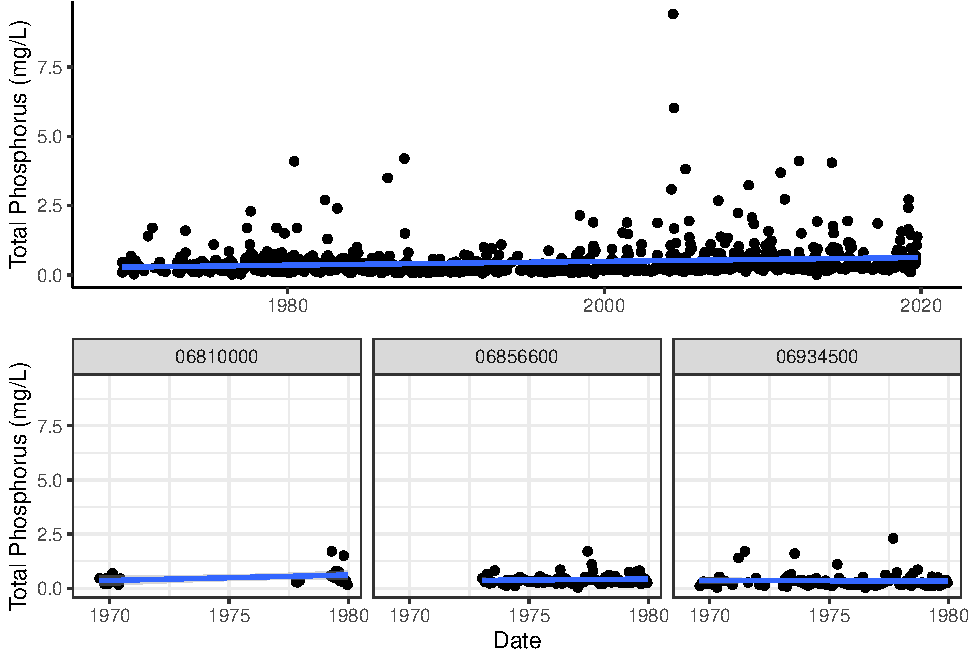
\includegraphics{Project_Template_files/figure-latex/tp.time-1.pdf}
\caption{\label{fig:tp.time}Total Phosphorus Over Time}
\end{figure}

As seen by \autoref{fig:tp.time}, total phosphorus values have a slight
positive trend. From \autoref{fig:tp.time}, site 06934500 has the most
total phosphorus data.

\begin{figure}
\centering
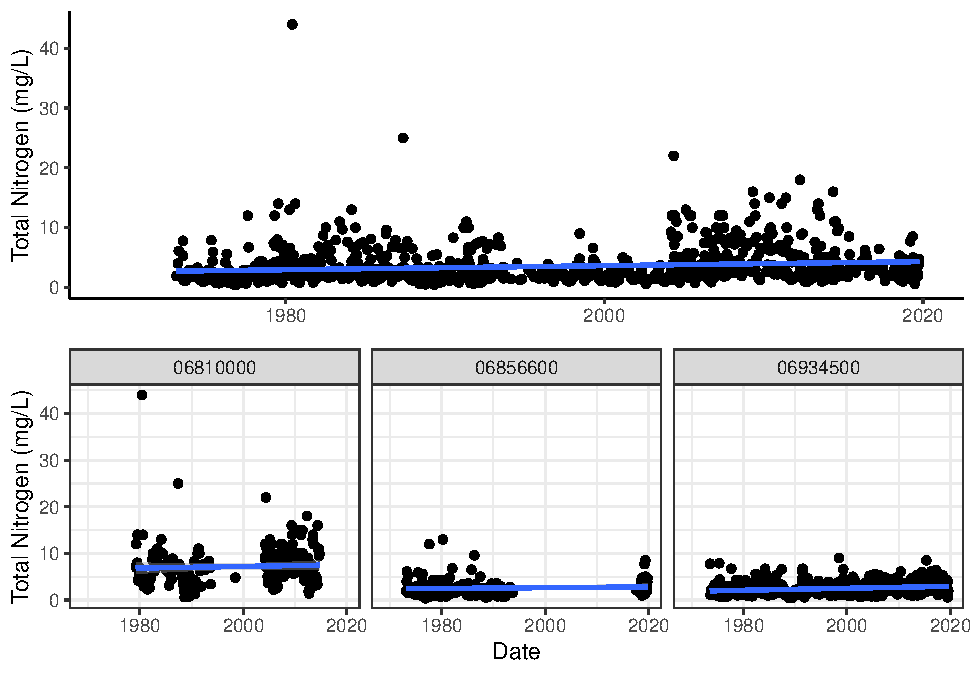
\includegraphics{Project_Template_files/figure-latex/tn.time-1.pdf}
\caption{\label{fig:tn.time}Total Nitrogen Over Time}
\end{figure}

From \autoref{fig:tn.time}, total nitrogen looks as though there is a
slight positive trend from 1980 to 2019. Again, site 06934500 has the
most total nitrogen data, as evidenced in \autoref{fig:tn.time}.

\begin{figure}
\centering
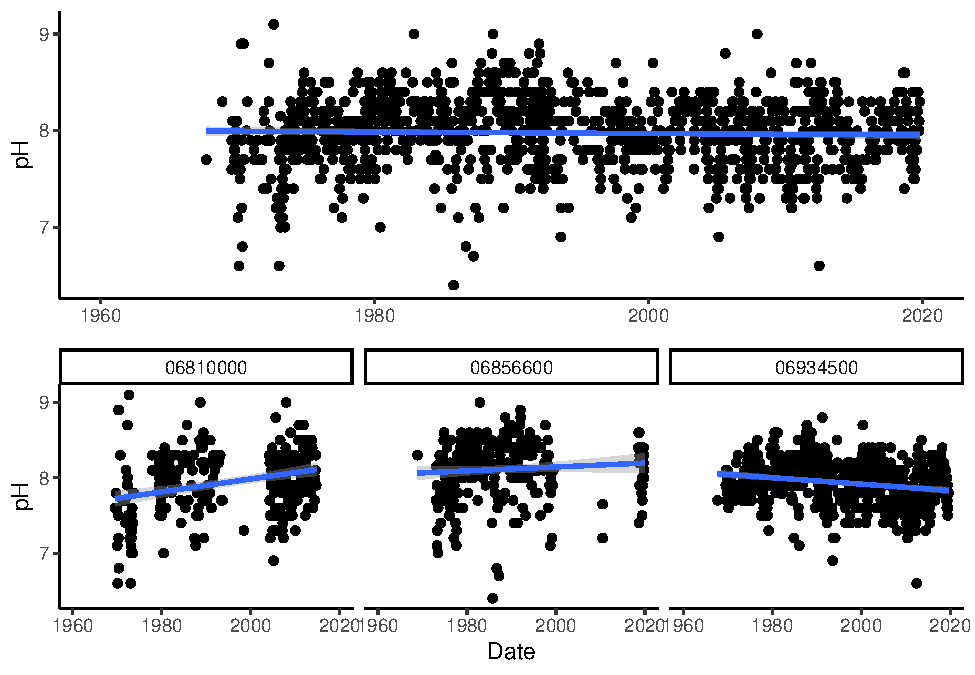
\includegraphics{Project_Template_files/figure-latex/ph-1.pdf}
\caption{\label{fig:ph}pH Over Time}
\end{figure}

As seen in \autoref{fig:ph}, pH values range from below pH of 7 to above
pH of 9 from 1970 - 2019. From \autoref{fig:ph}, site 06810000 has a
positive increase in pH over time, whereas site 06934500 has a
decreasing trend in pH over time.

\begin{figure}
\centering
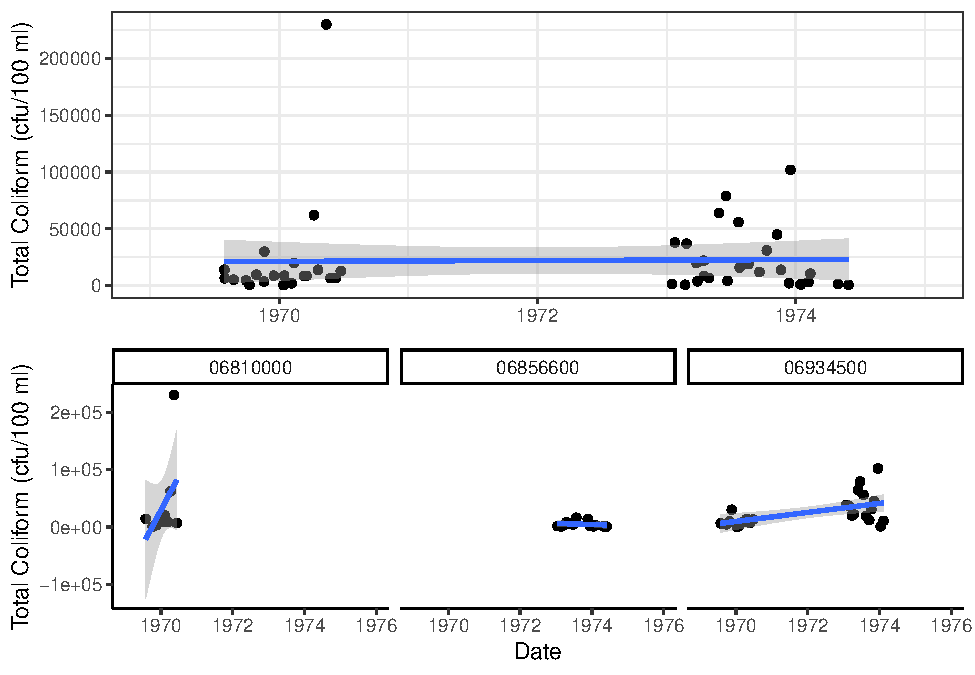
\includegraphics{Project_Template_files/figure-latex/tc.time-1.pdf}
\caption{\label{fig:tc.time}Total Coliform Over Time}
\end{figure}

\autoref{fig:tc.time} shows the total coliform measurements in the 3
chosen sites over time. From \autoref{fig:tc.time}, it is evident that
there is not much data on total coliform in the Missouri River Basin and
monitoring for total coliform occured at these 3 sites from late 1960s
through 1975.

\begin{figure}
\centering
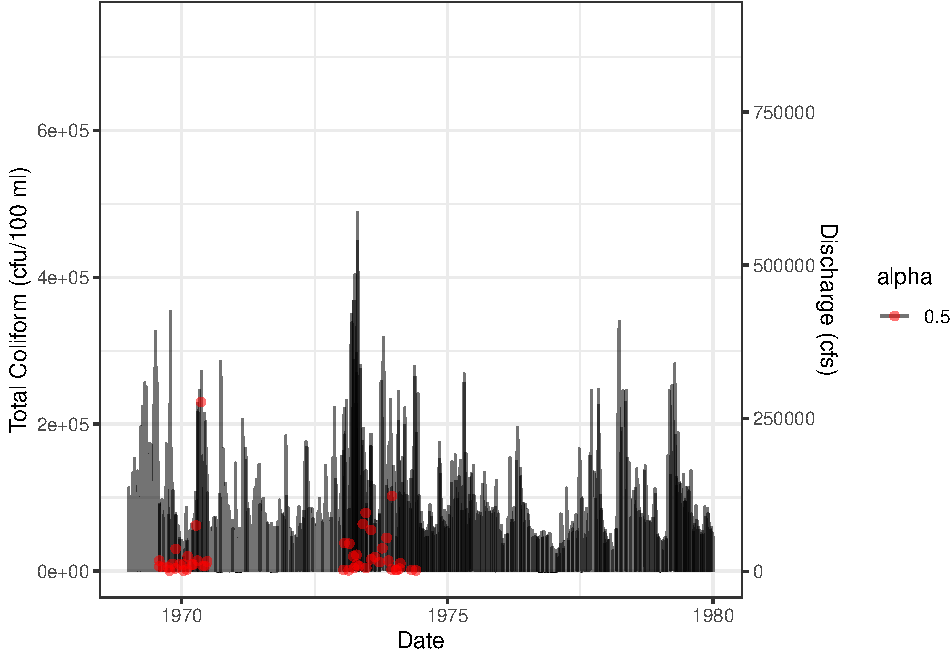
\includegraphics{Project_Template_files/figure-latex/tc.dis-1.pdf}
\caption{\label{fig:tc.dis}Total Coliform over time and Discharge over
time}
\end{figure}

\autoref{fig:tc.dis} was created to determine whether high amounts of
total coliform coincided with an increase in discharge. Because there
were limited total coliform measurements taken, as evidenced in
\autoref{fig:tc.time}, there is not a great conclusion from this data.
However, \autoref{fig:tc.dis} shows a spike in discharge events between
1972 - 1974, which also happens to be a time when total coliform was
sampled. \autoref{fig:tc.dis} also shows increases in total coliform
between 1972 - 1975.

\newpage

\hypertarget{time-series-analysis}{%
\subsubsection{Time Series Analysis}\label{time-series-analysis}}

In time series analysis, we focus on the same 3 sites chosen in the
water quality analysis.

\begin{Shaded}
\begin{Highlighting}[]
\CommentTok{#Discharge Data}
\CommentTok{# 06810000 Nishnabotna River above Hamburg, IA }
\NormalTok{NRHDischarge <-}\StringTok{ }\KeywordTok{readNWISdv}\NormalTok{(}\DataTypeTok{siteNumbers =} \StringTok{"06810000"}\NormalTok{,}
                           \DataTypeTok{parameterCd =} \StringTok{"00060"}\NormalTok{, }\CommentTok{# discharge (ft3/s)}
                           \DataTypeTok{startDate =} \StringTok{""}\NormalTok{,}
                           \DataTypeTok{endDate =} \StringTok{""}\NormalTok{)}
\KeywordTok{names}\NormalTok{(NRHDischarge)[}\DecValTok{4}\OperatorTok{:}\DecValTok{5}\NormalTok{] <-}\KeywordTok{c}\NormalTok{(}\StringTok{"Discharge"}\NormalTok{, }\StringTok{"Approval.Code"}\NormalTok{)}
\CommentTok{# 06934500 Missouri River at Hermann, MO}
\NormalTok{MRHDischarge <-}\StringTok{ }\KeywordTok{readNWISdv}\NormalTok{(}\DataTypeTok{siteNumbers =} \StringTok{"06934500"}\NormalTok{,}
                             \DataTypeTok{parameterCd =} \StringTok{"00060"}\NormalTok{, }\CommentTok{# discharge (ft3/s)}
                             \DataTypeTok{startDate =} \StringTok{""}\NormalTok{,}
                             \DataTypeTok{endDate =} \StringTok{""}\NormalTok{)}
\KeywordTok{names}\NormalTok{(MRHDischarge)[}\DecValTok{4}\OperatorTok{:}\DecValTok{5}\NormalTok{] <-}\KeywordTok{c}\NormalTok{(}\StringTok{"Discharge"}\NormalTok{, }\StringTok{"Approval.Code"}\NormalTok{)}
\CommentTok{# 06856600 REPUBLICAN R AT CLAY CENTER, KS}
\NormalTok{RRCCDischarge <-}\StringTok{ }\KeywordTok{readNWISdv}\NormalTok{(}\DataTypeTok{siteNumbers =} \StringTok{"06856600"}\NormalTok{,}
                           \DataTypeTok{parameterCd =} \StringTok{"00060"}\NormalTok{, }\CommentTok{# discharge (ft3/s)}
                           \DataTypeTok{startDate =} \StringTok{""}\NormalTok{,}
                           \DataTypeTok{endDate =} \StringTok{""}\NormalTok{)}
\KeywordTok{names}\NormalTok{(RRCCDischarge)[}\DecValTok{4}\OperatorTok{:}\DecValTok{5}\NormalTok{] <-}\KeywordTok{c}\NormalTok{(}\StringTok{"Discharge"}\NormalTok{, }\StringTok{"Approval.Code"}\NormalTok{)}

\CommentTok{# Nitrogen Data}
\CommentTok{# 06810000 Nishnabotna River above Hamburg, IA }
\NormalTok{NRHNitrogen <-}\StringTok{ }\KeywordTok{readNWISqw}\NormalTok{(}\DataTypeTok{siteNumbers =} \StringTok{"06810000"}\NormalTok{,}
                          \DataTypeTok{parameterCd =} \StringTok{"00600"}\NormalTok{, }\CommentTok{# nitrogen (mg/L)}
                          \DataTypeTok{startDate =} \StringTok{""}\NormalTok{,}
                          \DataTypeTok{endDate =} \StringTok{""}\NormalTok{) }\OperatorTok
\StringTok{  }\KeywordTok{select}\NormalTok{(sample_dt, result_va)}
\CommentTok{# 06934500 Missouri River at Hermann, MO}
\NormalTok{MRHNitrogen <-}\StringTok{ }\KeywordTok{readNWISqw}\NormalTok{(}\DataTypeTok{siteNumbers =} \StringTok{"06934500"}\NormalTok{,}
                            \DataTypeTok{parameterCd =} \StringTok{"00600"}\NormalTok{, }\CommentTok{# nitrogen (mg/L)}
                            \DataTypeTok{startDate =} \StringTok{""}\NormalTok{,}
                            \DataTypeTok{endDate =} \StringTok{""}\NormalTok{) }\OperatorTok
\StringTok{  }\KeywordTok{select}\NormalTok{(sample_dt, result_va)}
\CommentTok{# 06856600 REPUBLICAN R AT CLAY CENTER, KS}
\NormalTok{RRCCNitrogen <-}\StringTok{ }\KeywordTok{readNWISqw}\NormalTok{(}\DataTypeTok{siteNumbers =} \StringTok{"06856600"}\NormalTok{,}
                          \DataTypeTok{parameterCd =} \StringTok{"00600"}\NormalTok{, }\CommentTok{# nitrogen (mg/L)}
                          \DataTypeTok{startDate =} \StringTok{""}\NormalTok{,}
                          \DataTypeTok{endDate =} \StringTok{""}\NormalTok{) }\OperatorTok
\StringTok{  }\KeywordTok{select}\NormalTok{(sample_dt, result_va)}

\CommentTok{#Phosphorus Data}
\CommentTok{# 06810000 Nishnabotna River above Hamburg, IA }
\NormalTok{NRHPhosphorus <-}\StringTok{ }\KeywordTok{readNWISqw}\NormalTok{(}\DataTypeTok{siteNumbers =} \StringTok{"06810000"}\NormalTok{,}
                            \DataTypeTok{parameterCd =} \StringTok{"00665"}\NormalTok{, }\CommentTok{# phosphorus (mg/L)}
                            \DataTypeTok{startDate =} \StringTok{""}\NormalTok{,}
                            \DataTypeTok{endDate =} \StringTok{""}\NormalTok{) }\OperatorTok
\StringTok{  }\KeywordTok{select}\NormalTok{(sample_dt, result_va)}
\CommentTok{# 06934500 Missouri River at Hermann, MO}
\NormalTok{MRHPhosphorus <-}\StringTok{ }\KeywordTok{readNWISqw}\NormalTok{(}\DataTypeTok{siteNumbers =} \StringTok{"06934500"}\NormalTok{,}
                              \DataTypeTok{parameterCd =} \StringTok{"00665"}\NormalTok{, }\CommentTok{# phosphorus (mg/L)}
                              \DataTypeTok{startDate =} \StringTok{""}\NormalTok{,}
                              \DataTypeTok{endDate =} \StringTok{""}\NormalTok{) }\OperatorTok
\StringTok{  }\KeywordTok{select}\NormalTok{(sample_dt, result_va)}
\CommentTok{# 06856600 REPUBLICAN R AT CLAY CENTER, KS}
\NormalTok{RRCCPhosphorus <-}\StringTok{ }\KeywordTok{readNWISqw}\NormalTok{(}\DataTypeTok{siteNumbers =} \StringTok{"06856600"}\NormalTok{,}
                            \DataTypeTok{parameterCd =} \StringTok{"00665"}\NormalTok{, }\CommentTok{# phosphorus (mg/L)}
                            \DataTypeTok{startDate =} \StringTok{""}\NormalTok{,}
                            \DataTypeTok{endDate =} \StringTok{""}\NormalTok{) }\OperatorTok
\StringTok{  }\KeywordTok{select}\NormalTok{(sample_dt, result_va)}
\end{Highlighting}
\end{Shaded}

\begin{figure}
\centering
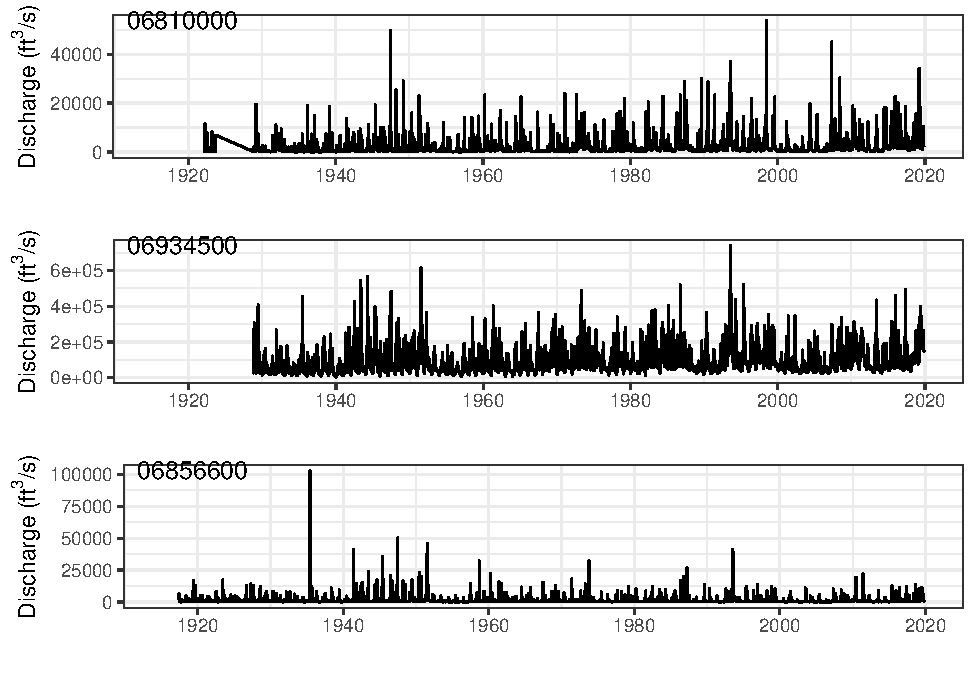
\includegraphics{Project_Template_files/figure-latex/discharge.time-1.pdf}
\caption{\label{fig:discharge.time}Discharge Over Time}
\end{figure}

As seen by \autoref{fig:discharge.time}, there is a gap of discharge
data in 06810000. Therefore, we filter the discharge data by the date
and only use the data available after 1928-01-01 for site 06810000.

\begin{figure}
\centering
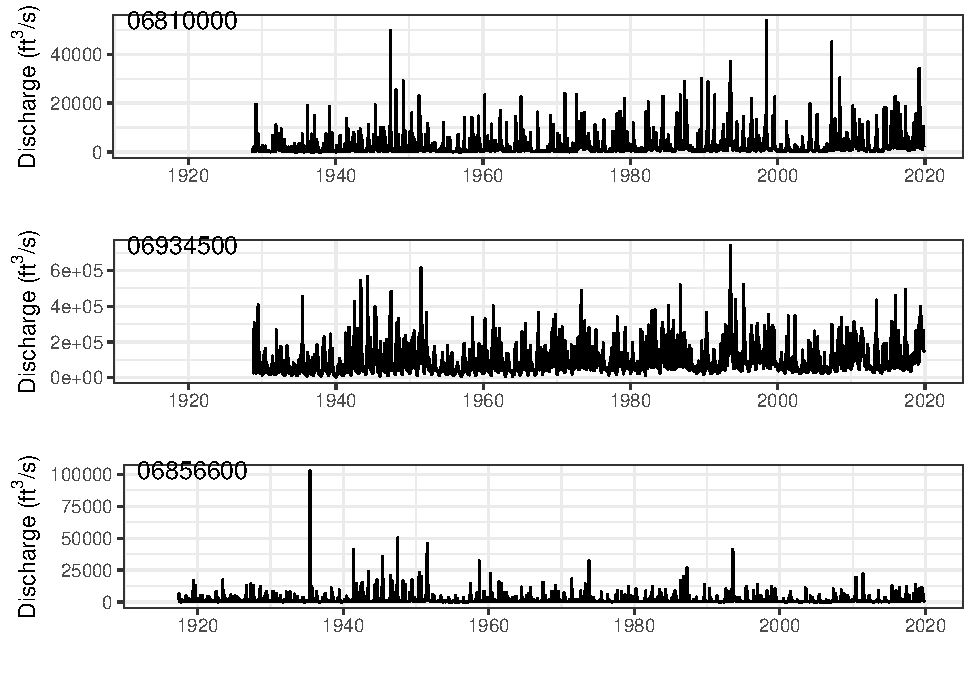
\includegraphics{Project_Template_files/figure-latex/dis.t3-1.pdf}
\caption{\label{fig:dis.t3}Discharge Over Time for 3 sites}
\end{figure}

Also, we do the same things for nitrogen and phosphorus.

\begin{figure}
\centering
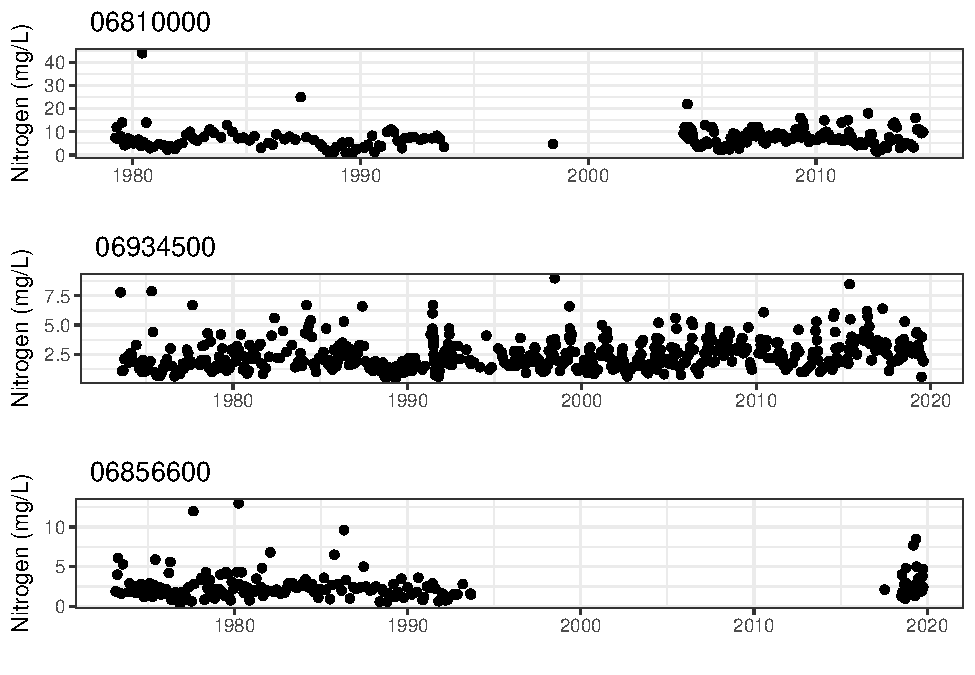
\includegraphics{Project_Template_files/figure-latex/N.t-1.pdf}
\caption{\label{fig:N.t}Nitrogen Over Time}
\end{figure}

\begin{figure}
\centering
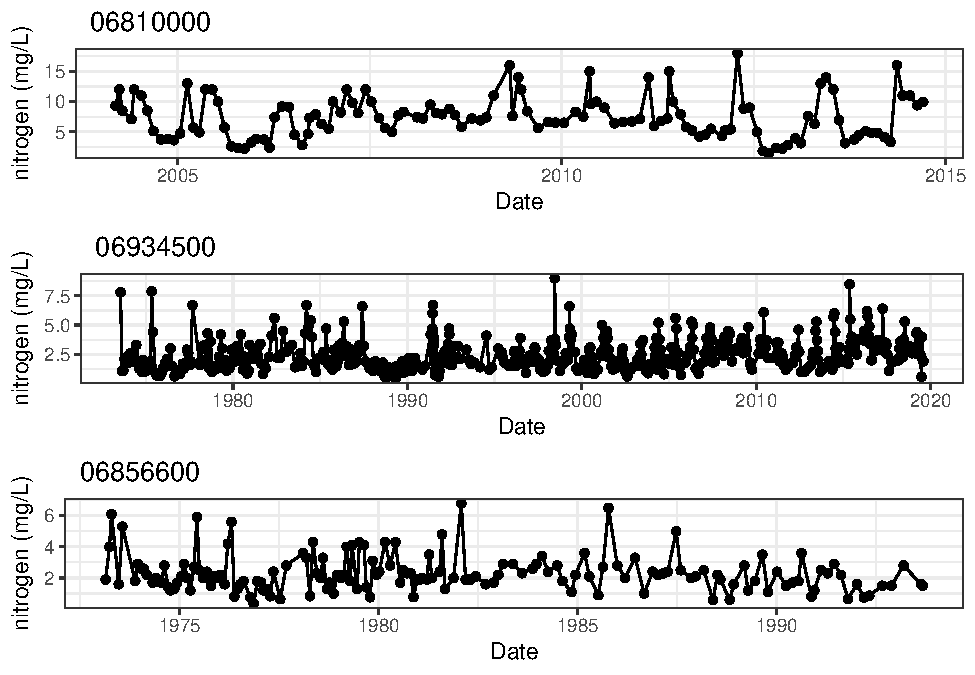
\includegraphics{Project_Template_files/figure-latex/N.t3-1.pdf}
\caption{\label{fig:N.t3}Nitrogen Over Time for 3 sites after filtering}
\end{figure}

\begin{figure}
\centering
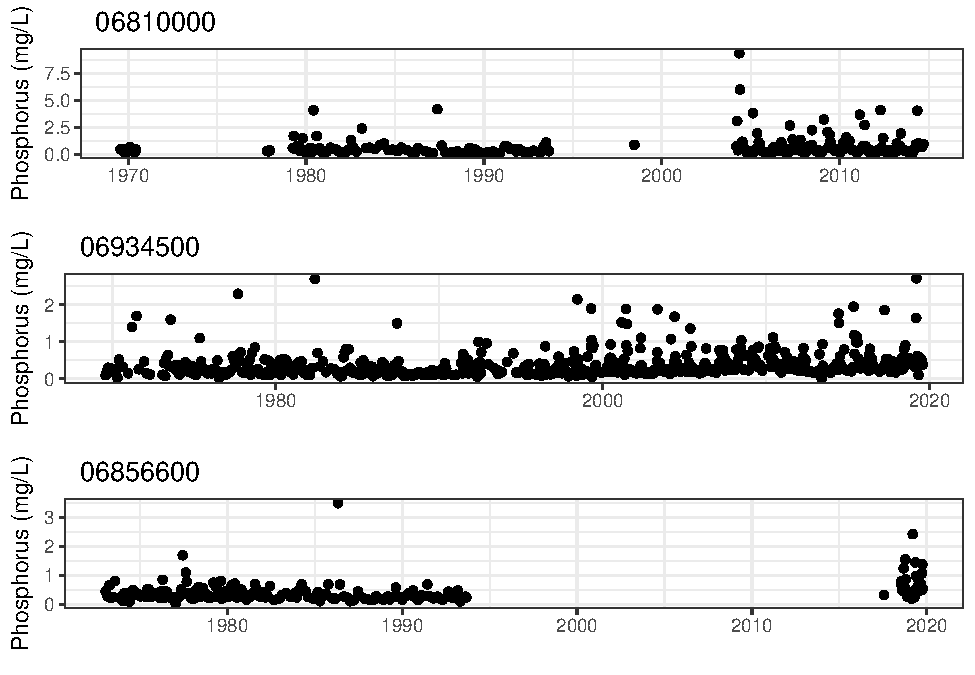
\includegraphics{Project_Template_files/figure-latex/P.t-1.pdf}
\caption{\label{fig:P.t}Phosphorus Over Time}
\end{figure}

\begin{figure}
\centering
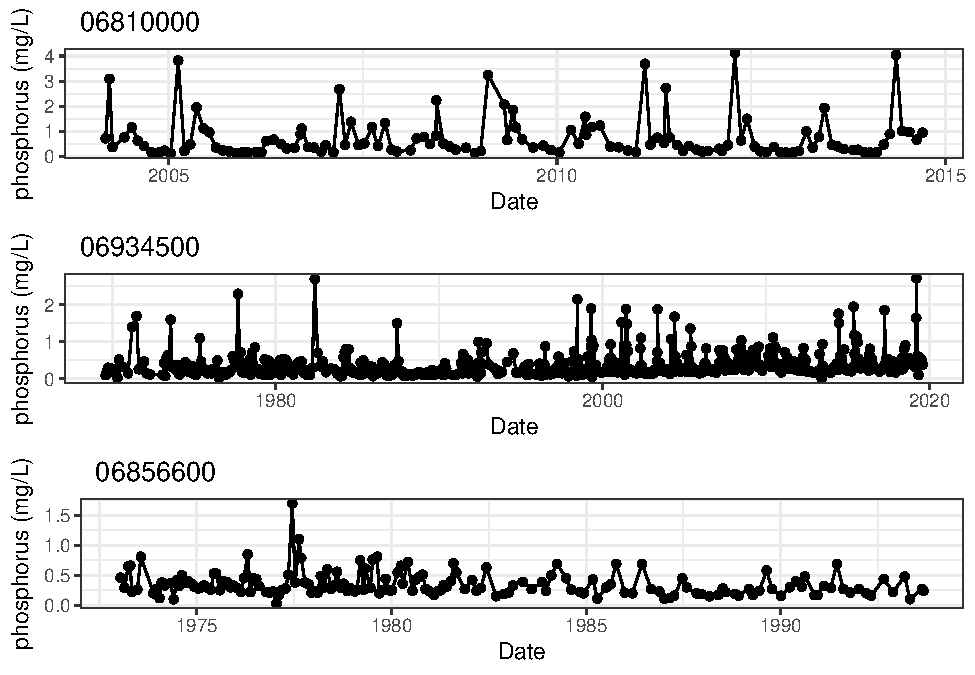
\includegraphics{Project_Template_files/figure-latex/P.t3-1.pdf}
\caption{\label{fig:P.t3}Phosphorus Over Time for 3 sites after
filtering}
\end{figure}

\hypertarget{high-frequency-nitrogen-and-discharge}{%
\subsection{High Frequency Nitrogen and
Discharge}\label{high-frequency-nitrogen-and-discharge}}

\begin{Shaded}
\begin{Highlighting}[]
\CommentTok{#high frequency data wrangling}
\NormalTok{highfreqsite2019 <-}\StringTok{ }\NormalTok{highfreqsiteinfo }\OperatorTok
\StringTok{  }\KeywordTok{filter}\NormalTok{(end_date }\OperatorTok{>}\StringTok{ "2019-03-31"}\NormalTok{); }\KeywordTok{head}\NormalTok{(highfreqsite2019)}
\end{Highlighting}
\end{Shaded}

\begin{verbatim}
## Warning in Ops.factor(end_date, "2019-03-31"): '>' not meaningful for
## factors
\end{verbatim}

\begin{verbatim}
##  [1] X                  agency_cd          site_no           
##  [4] station_nm         site_tp_cd         dec_lat_va        
##  [7] dec_long_va        coord_acy_cd       dec_coord_datum_cd
## [10] alt_va             alt_acy_va         alt_datum_cd      
## [13] huc_cd             data_type_cd       parm_cd           
## [16] stat_cd            ts_id              loc_web_ds        
## [19] medium_grp_cd      parm_grp_cd        srs_id            
## [22] access_cd          begin_date         end_date          
## [25] count_nu          
## <0 rows> (or 0-length row.names)
\end{verbatim}

\begin{Shaded}
\begin{Highlighting}[]
\NormalTok{highfreqsites.DN <-}\StringTok{ }\KeywordTok{readNWISuv}\NormalTok{(}\DataTypeTok{site =} \KeywordTok{c}\NormalTok{(}\StringTok{"06808500"}\NormalTok{, }\StringTok{"06817000"}\NormalTok{, }\StringTok{"06892350"}\NormalTok{, }\StringTok{"06934500"}\NormalTok{), }
                               \DataTypeTok{parameterCd =} \KeywordTok{c}\NormalTok{(}\StringTok{"00060"}\NormalTok{, }\StringTok{"99133"}\NormalTok{), }
                               \CommentTok{# Discharge in cfs & Nitrate in mg/l NO3-N}
                               \DataTypeTok{startDate =} \StringTok{"2019-01-01"}\NormalTok{,}
                               \DataTypeTok{endDate =} \StringTok{"2019-11-01"}\NormalTok{) }\OperatorTok
\StringTok{                               }\KeywordTok{renameNWISColumns}\NormalTok{() }\OperatorTok
\StringTok{                               }\KeywordTok{rename}\NormalTok{(}\DataTypeTok{Nitrate_mgl =} \DecValTok{6}\NormalTok{)}

\CommentTok{#individual sites}
\NormalTok{Hermann <-}\StringTok{ }\NormalTok{highfreqsites.DN }\OperatorTok
\StringTok{           }\KeywordTok{filter}\NormalTok{(site_no}\OperatorTok{==}\StringTok{"06934500"}\NormalTok{)}
\NormalTok{Desoto <-}\StringTok{ }\NormalTok{highfreqsites.DN }\OperatorTok
\StringTok{          }\KeywordTok{filter}\NormalTok{(site_no}\OperatorTok{==}\StringTok{"06892350"}\NormalTok{)}
\NormalTok{Clarinda <-}\StringTok{ }\NormalTok{highfreqsites.DN }\OperatorTok
\StringTok{            }\KeywordTok{filter}\NormalTok{(site_no}\OperatorTok{==}\StringTok{"06817000"}\NormalTok{)}
\NormalTok{Randolph <-}\StringTok{ }\NormalTok{highfreqsites.DN }\OperatorTok
\StringTok{            }\KeywordTok{filter}\NormalTok{(site_no}\OperatorTok{==}\StringTok{"06808500"}\NormalTok{)}
\end{Highlighting}
\end{Shaded}

There were 7 sites in our region of interest that had high freq N data,
and only 4 sites had high freq N data during the floods of 2019. The
sites looked at in depth are:

\begin{verbatim}
- West Nishnabotna River in Randolph, IA
- Nodaway River at Clarinda, IA
- Kansas River in Desoto, KS
- Missouri River at Hermann, MO
\end{verbatim}

The Missouri River is the biggest river, with an average of 214693 cfs
discharge rate during the year 2019, and the Nodaway River is the
smallest river, with an average of 1185 cfs discharge rate for 2019.

In March of 2019, a
\href{https://www.kansascity.com/news/state/missouri/article228237519.html}{bomb
cyclone} hit the midwest. Our initial research question, what effect did
the March 2019 storm have on water quality, attempted to look into the
behavior of nitrogen in the discharge of the rivers. Unfortunately,
instantaneous Nitrogen values stopped recording during the peak of the
storm events in March, so it was hard to create hysteresis plots that
exhibited the type of storm and its effects on nitrogen concentration.

Even though Nitrogen concentrations were not recorded in March, they
were recorded in other times of the year. 2019 was a wet year and many
large storm events occurred.

\begin{verbatim}
## Warning: Removed 9 rows containing missing values (geom_point).
\end{verbatim}

\begin{figure}
\centering
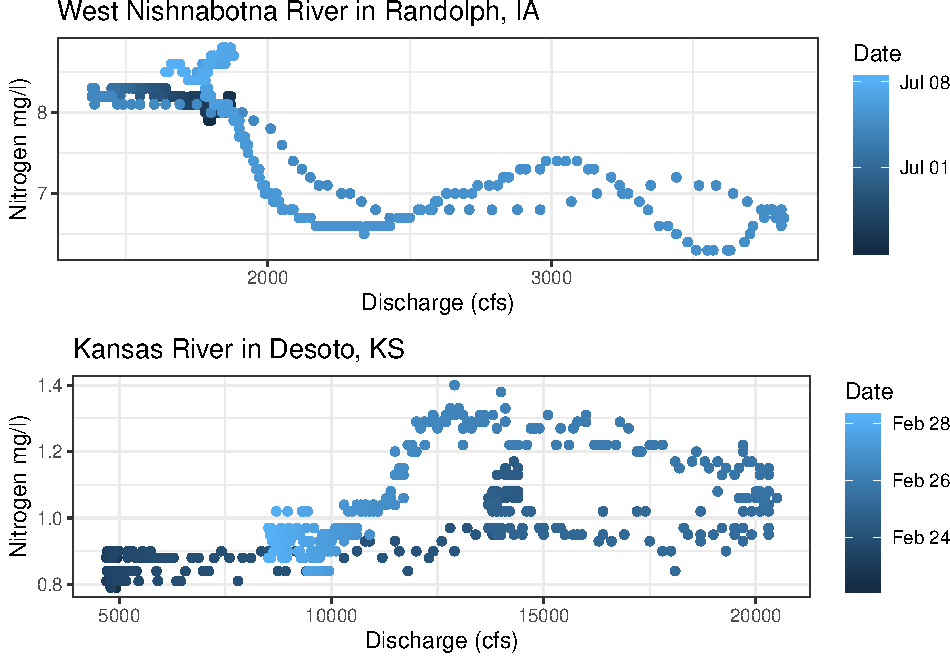
\includegraphics{Project_Template_files/figure-latex/desotos-1.pdf}
\caption{\label{fig:desotos} Hysteresis plots}
\end{figure}

The \autoref{fig:desotos} shows Hysteresis plots for two storm events in
the Missouri River Basin. The storm event on the West Nishnabotna River
exhibits an oddly-shaped plot that has a negative slope, indicating it
is a diluting storm. The Kansas River experienced a storm in late
February that has a counter-clockwise motion and a positive slope,
indicating a flushing storm. These two plots illustrate that two rivers
near each other can have very different behaviors.

\newpage

\hypertarget{analysis}{%
\section{Analysis}\label{analysis}}

\hypertarget{linear-models-for-water-quality}{%
\subsection{Linear Models for Water
Quality}\label{linear-models-for-water-quality}}

Linear models were run for total nitrogen, total phosphorus, total
coliform, and pH to determine if there were significant patterns in the
data.

\begin{verbatim}
## 
## Call:
## lm(formula = total.nitrogen ~ Date, data = bestsites.wq.skinny)
## 
## Residuals:
##    Min     1Q Median     3Q    Max 
## -3.708 -1.709 -0.917  0.524 41.040 
## 
## Coefficients:
##              Estimate Std. Error t value Pr(>|t|)    
## (Intercept) 2.605e+00  2.082e-01  12.517  < 2e-16 ***
## Date        9.310e-05  1.928e-05   4.828  1.6e-06 ***
## ---
## Signif. codes:  0 '***' 0.001 '**' 0.01 '*' 0.05 '.' 0.1 ' ' 1
## 
## Residual standard error: 3.051 on 992 degrees of freedom
##   (104765 observations deleted due to missingness)
## Multiple R-squared:  0.02296,    Adjusted R-squared:  0.02197 
## F-statistic: 23.31 on 1 and 992 DF,  p-value: 1.598e-06
\end{verbatim}

\begin{verbatim}
## 
## Call:
## lm(formula = total.coliform ~ Date, data = bestsites.wq.skinny)
## 
## Residuals:
##    Min     1Q Median     3Q    Max 
## -22343 -18568 -12589  -1235 208472 
## 
## Coefficients:
##              Estimate Std. Error t value Pr(>|t|)  
## (Intercept) 21389.217   8351.431   2.561   0.0138 *
## Date            1.046      8.329   0.126   0.9006  
## ---
## Signif. codes:  0 '***' 0.001 '**' 0.01 '*' 0.05 '.' 0.1 ' ' 1
## 
## Residual standard error: 38270 on 46 degrees of freedom
##   (105711 observations deleted due to missingness)
## Multiple R-squared:  0.0003425,  Adjusted R-squared:  -0.02139 
## F-statistic: 0.01576 on 1 and 46 DF,  p-value: 0.9006
\end{verbatim}

\begin{verbatim}
## 
## Call:
## lm(formula = total.phosphorus ~ Date, data = bestsites.wq.skinny)
## 
## Residuals:
##     Min      1Q  Median      3Q     Max 
## -0.5768 -0.2685 -0.1320  0.0578  8.8856 
## 
## Coefficients:
##              Estimate Std. Error t value Pr(>|t|)    
## (Intercept) 2.876e-01  3.570e-02   8.055 2.14e-15 ***
## Date        1.887e-05  3.394e-06   5.561 3.40e-08 ***
## ---
## Signif. codes:  0 '***' 0.001 '**' 0.01 '*' 0.05 '.' 0.1 ' ' 1
## 
## Residual standard error: 0.5752 on 1048 degrees of freedom
##   (104709 observations deleted due to missingness)
## Multiple R-squared:  0.02866,    Adjusted R-squared:  0.02774 
## F-statistic: 30.92 on 1 and 1048 DF,  p-value: 3.404e-08
\end{verbatim}

\begin{verbatim}
## 
## Call:
## lm(formula = pH ~ Date, data = bestsites.wq.skinny)
## 
## Residuals:
##      Min       1Q   Median       3Q      Max 
## -1.57958 -0.18708  0.02653  0.23034  1.11246 
## 
## Coefficients:
##               Estimate Std. Error t value Pr(>|t|)    
## (Intercept)  7.989e+00  1.973e-02 404.824   <2e-16 ***
## Date        -1.660e-06  1.938e-06  -0.856    0.392    
## ---
## Signif. codes:  0 '***' 0.001 '**' 0.01 '*' 0.05 '.' 0.1 ' ' 1
## 
## Residual standard error: 0.355 on 1199 degrees of freedom
##   (104558 observations deleted due to missingness)
## Multiple R-squared:  0.0006111,  Adjusted R-squared:  -0.0002224 
## F-statistic: 0.7331 on 1 and 1199 DF,  p-value: 0.392
\end{verbatim}

Linear models were created in order to determine whether water quality
parameters have changed over time. When nitrogen was evaluated for all
sites over the time period, it was found that nitrogen has significantly
increased over time (p\textless{} 2e-16, F\_\{1,992\} = 23.31). At the
six sites that total coliform was recorded, total coliform significantly
increased over the time period (p \textless{} 0.0138, F\_\{1,46\} =
0.01576). However, this result should be critically analyzed, because
total coliform has not been measured since the 1980s. Total coliform
levels should be measured more closely in this region, given the lack of
data. A linear model was also performed on total phosphorus over time,
and it was found that phosphorus levels have also increased over the
time period for all sites of interest (p \textless{} 2.14e-15,
F\_\{1,1048\} = 30.92). Lastly, pH was analyzed in a linear model and it
was found that pH had no significant increase or decrease over time in
all of the sites of interest (p = 0.392).

A time series analysis will be conducted on the discharge from the
chosen sies. This will include an analysis of baseflow and quickflow. A
dygraph of discharge over time will be created to be able to better
examine large increases in discharge.

For high frequency data, a hystersis plot will be created to determine
hydrologic flashiness.

\newpage

\begin{Shaded}
\begin{Highlighting}[]
\CommentTok{##Time Series}

\CommentTok{# 06810000 Nishnabotna River above Hamburg, IA }

\CommentTok{########################### Discharge Analysis ############################}
\NormalTok{NRHRegressionPlot <-}\StringTok{ }
\StringTok{  }\KeywordTok{ggplot}\NormalTok{(NRHDischarge, }\KeywordTok{aes}\NormalTok{(}\DataTypeTok{x =}\NormalTok{ Date, }\DataTypeTok{y =}\NormalTok{ Discharge)) }\OperatorTok{+}
\StringTok{  }\KeywordTok{geom_line}\NormalTok{() }\OperatorTok{+}
\StringTok{  }\KeywordTok{geom_smooth}\NormalTok{(}\DataTypeTok{method =} \StringTok{"lm"}\NormalTok{, }\DataTypeTok{se =} \OtherTok{FALSE}\NormalTok{, }\DataTypeTok{color =} \StringTok{"#c13d75ff"}\NormalTok{) }\OperatorTok{+}
\StringTok{  }\KeywordTok{labs}\NormalTok{(}\DataTypeTok{x =} \StringTok{""}\NormalTok{, }\DataTypeTok{y =} \KeywordTok{expression}\NormalTok{(}\StringTok{"Discharge (ft"}\OperatorTok{^}\DecValTok{3}\OperatorTok{*}\StringTok{"/s)"}\NormalTok{)) }\OperatorTok{+}\StringTok{ }
\StringTok{  }\KeywordTok{theme}\NormalTok{(}\DataTypeTok{plot.title =} \KeywordTok{element_text}\NormalTok{(}\DataTypeTok{margin =} \KeywordTok{margin}\NormalTok{(}\DataTypeTok{b =} \DecValTok{-10}\NormalTok{), }\DataTypeTok{size =} \DecValTok{12}\NormalTok{), }
        \DataTypeTok{axis.title.x =} \KeywordTok{element_blank}\NormalTok{())}
\KeywordTok{print}\NormalTok{(NRHRegressionPlot)}
\end{Highlighting}
\end{Shaded}

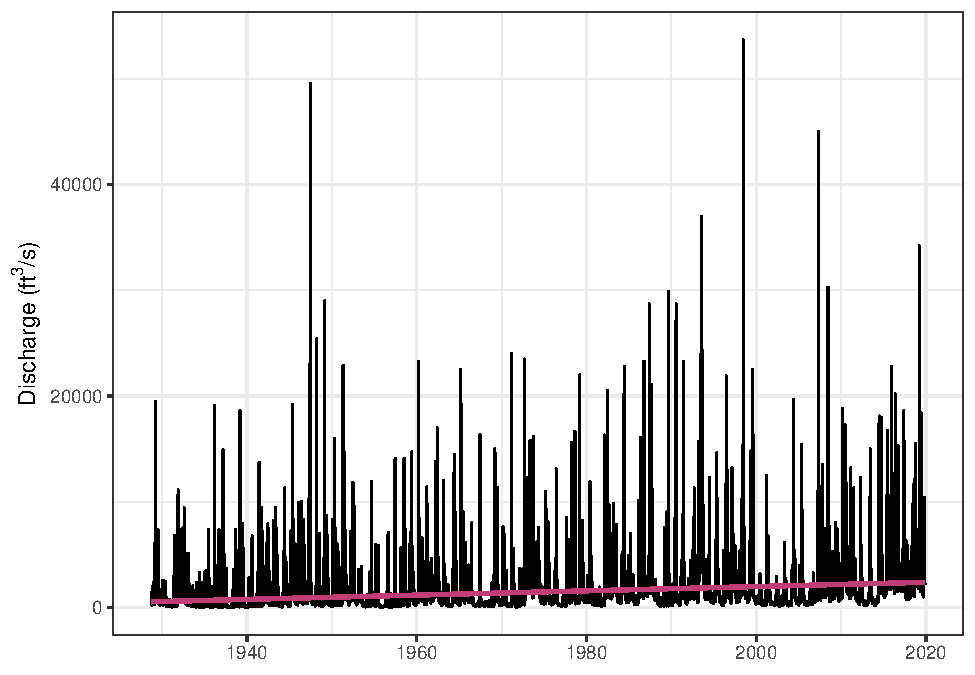
\includegraphics{Project_Template_files/figure-latex/unnamed-chunk-6-1.pdf}

\begin{Shaded}
\begin{Highlighting}[]
\NormalTok{NRHDischarge <-}\StringTok{ }\KeywordTok{na.omit}\NormalTok{(NRHDischarge)}
\NormalTok{NRH_ts <-}\StringTok{ }\KeywordTok{ts}\NormalTok{(NRHDischarge[[}\DecValTok{4}\NormalTok{]], }\DataTypeTok{frequency =} \DecValTok{365}\NormalTok{)}
\KeywordTok{table}\NormalTok{(}\KeywordTok{diff}\NormalTok{(NRHDischarge}\OperatorTok{$}\NormalTok{Date))}
\end{Highlighting}
\end{Shaded}

\begin{verbatim}
## 
##     1 
## 33279
\end{verbatim}

\begin{Shaded}
\begin{Highlighting}[]
\CommentTok{# Generate the decomposition}
\NormalTok{NRH_Decomposed <-}\StringTok{ }\KeywordTok{stl}\NormalTok{(NRH_ts, }\DataTypeTok{s.window =} \StringTok{"periodic"}\NormalTok{)}

\CommentTok{# Visualize the decomposed series. }
\KeywordTok{plot}\NormalTok{(NRH_Decomposed)}
\end{Highlighting}
\end{Shaded}

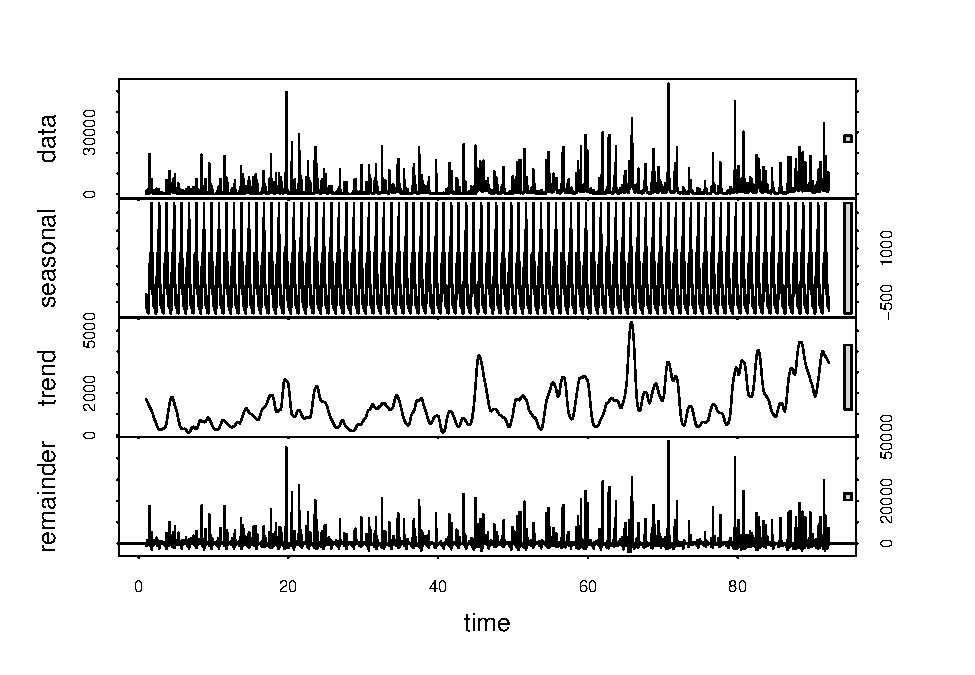
\includegraphics{Project_Template_files/figure-latex/unnamed-chunk-6-2.pdf}

\begin{Shaded}
\begin{Highlighting}[]
\CommentTok{# We can extract the components and turn them into data frames}
\NormalTok{NRH_Components <-}\StringTok{ }\KeywordTok{as.data.frame}\NormalTok{(NRH_Decomposed}\OperatorTok{$}\NormalTok{time.series[,}\DecValTok{1}\OperatorTok{:}\DecValTok{3}\NormalTok{])}
\NormalTok{NRH_Components <-}\StringTok{ }\KeywordTok{mutate}\NormalTok{(NRH_Components,}
                         \DataTypeTok{Observed =}\NormalTok{ NRHDischarge}\OperatorTok{$}\NormalTok{Discharge,     }
                         \DataTypeTok{Date =}\NormalTok{ NRHDischarge}\OperatorTok{$}\NormalTok{Date)}

\CommentTok{# Visualize how the trend maps onto the data}
\KeywordTok{ggplot}\NormalTok{(NRH_Components) }\OperatorTok{+}
\StringTok{  }\KeywordTok{geom_line}\NormalTok{(}\KeywordTok{aes}\NormalTok{(}\DataTypeTok{y =}\NormalTok{ Observed, }\DataTypeTok{x =}\NormalTok{ Date),  }\DataTypeTok{size =} \FloatTok{0.25}\NormalTok{) }\OperatorTok{+}
\StringTok{  }\KeywordTok{geom_line}\NormalTok{(}\KeywordTok{aes}\NormalTok{(}\DataTypeTok{y =}\NormalTok{ trend, }\DataTypeTok{x =}\NormalTok{ Date), }\DataTypeTok{color =} \StringTok{"#c13d75ff"}\NormalTok{) }\OperatorTok{+}
\StringTok{  }\KeywordTok{geom_hline}\NormalTok{(}\DataTypeTok{yintercept =} \DecValTok{0}\NormalTok{, }\DataTypeTok{lty =} \DecValTok{2}\NormalTok{) }\OperatorTok{+}
\StringTok{  }\KeywordTok{ylab}\NormalTok{(}\KeywordTok{expression}\NormalTok{(}\StringTok{"Discharge (ft"}\OperatorTok{^}\DecValTok{3}\OperatorTok{*}\StringTok{"/s)"}\NormalTok{))}
\end{Highlighting}
\end{Shaded}

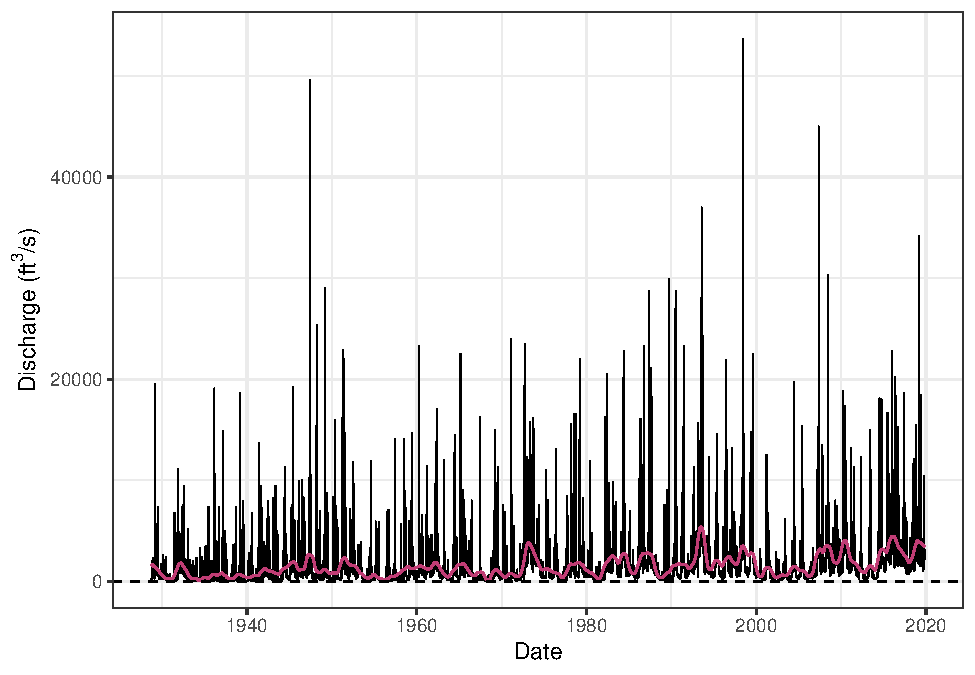
\includegraphics{Project_Template_files/figure-latex/unnamed-chunk-6-3.pdf}

\begin{Shaded}
\begin{Highlighting}[]
\CommentTok{# Visualize how the seasonal cycle maps onto the data}
\KeywordTok{ggplot}\NormalTok{(NRH_Components) }\OperatorTok{+}
\StringTok{  }\KeywordTok{geom_line}\NormalTok{(}\KeywordTok{aes}\NormalTok{(}\DataTypeTok{y =}\NormalTok{ Observed, }\DataTypeTok{x =}\NormalTok{ Date),  }\DataTypeTok{size =} \FloatTok{0.25}\NormalTok{) }\OperatorTok{+}
\StringTok{  }\KeywordTok{geom_line}\NormalTok{(}\KeywordTok{aes}\NormalTok{(}\DataTypeTok{y =}\NormalTok{ seasonal, }\DataTypeTok{x =}\NormalTok{ Date), }\DataTypeTok{color =} \StringTok{"#c13d75ff"}\NormalTok{) }\OperatorTok{+}
\StringTok{  }\KeywordTok{geom_hline}\NormalTok{(}\DataTypeTok{yintercept =} \DecValTok{0}\NormalTok{, }\DataTypeTok{lty =} \DecValTok{2}\NormalTok{) }\OperatorTok{+}
\StringTok{  }\KeywordTok{ylab}\NormalTok{(}\KeywordTok{expression}\NormalTok{(}\StringTok{"Discharge (ft"}\OperatorTok{^}\DecValTok{3}\OperatorTok{*}\StringTok{"/s)"}\NormalTok{))}
\end{Highlighting}
\end{Shaded}

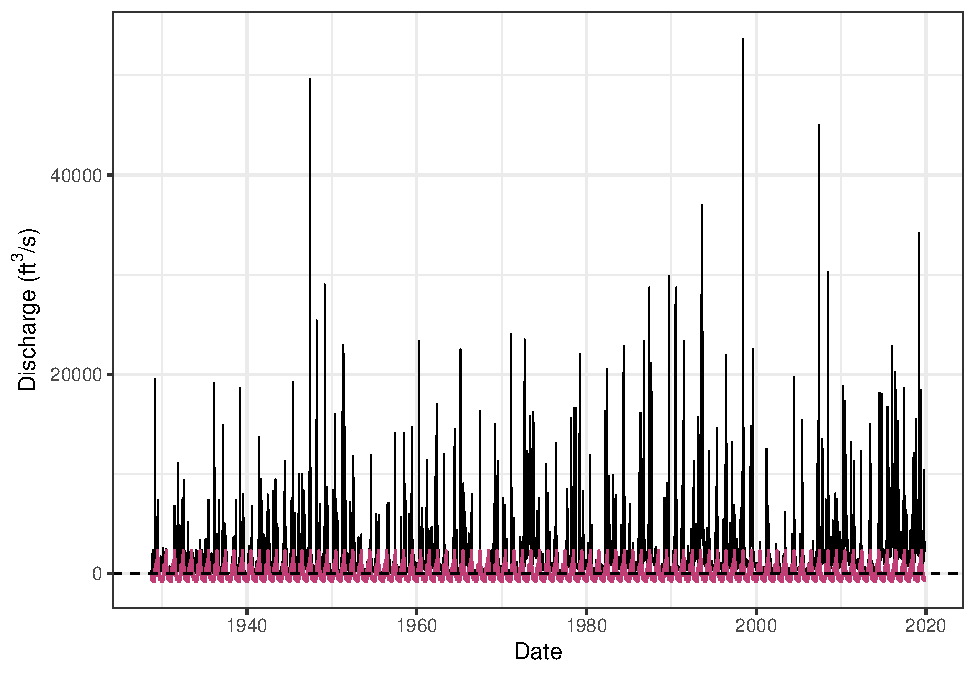
\includegraphics{Project_Template_files/figure-latex/unnamed-chunk-6-4.pdf}

\begin{Shaded}
\begin{Highlighting}[]
\NormalTok{NRHDischarge.Monthly <-}\StringTok{ }\NormalTok{NRHDischarge }\OperatorTok
\StringTok{  }\KeywordTok{mutate}\NormalTok{(}\DataTypeTok{Year =} \KeywordTok{year}\NormalTok{(Date),}
         \DataTypeTok{Month =} \KeywordTok{month}\NormalTok{(Date)) }\OperatorTok
\StringTok{  }\KeywordTok{group_by}\NormalTok{(Year, Month) }\OperatorTok
\StringTok{  }\KeywordTok{summarise}\NormalTok{(}\DataTypeTok{Discharge =} \KeywordTok{mean}\NormalTok{(Discharge))}
\NormalTok{NRHMonthly_ts <-}\StringTok{ }\KeywordTok{ts}\NormalTok{(NRHDischarge.Monthly[[}\DecValTok{3}\NormalTok{]], }\DataTypeTok{frequency =} \DecValTok{12}\NormalTok{)}
\KeywordTok{adf.test}\NormalTok{(NRHMonthly_ts, }\DataTypeTok{alternative =} \StringTok{"stationary"}\NormalTok{)}
\end{Highlighting}
\end{Shaded}

\begin{verbatim}
## Warning in adf.test(NRHMonthly_ts, alternative = "stationary"): p-value
## smaller than printed p-value
\end{verbatim}

\begin{verbatim}
## 
##  Augmented Dickey-Fuller Test
## 
## data:  NRHMonthly_ts
## Dickey-Fuller = -7.0535, Lag order = 10, p-value = 0.01
## alternative hypothesis: stationary
\end{verbatim}

\begin{Shaded}
\begin{Highlighting}[]
\KeywordTok{acf}\NormalTok{(NRHMonthly_ts)}
\end{Highlighting}
\end{Shaded}

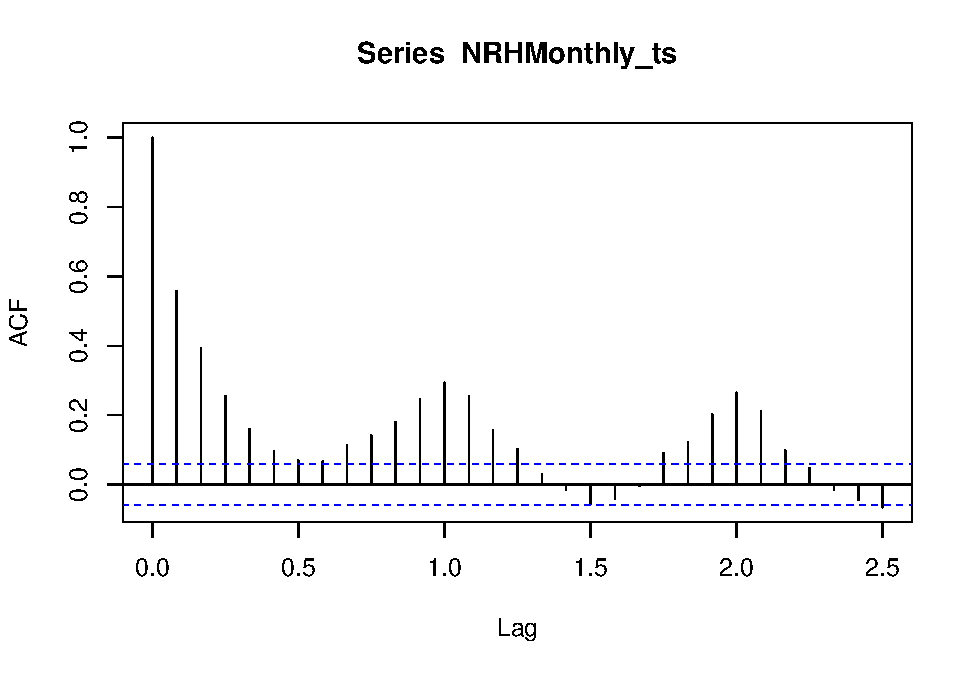
\includegraphics{Project_Template_files/figure-latex/unnamed-chunk-6-5.pdf}

\begin{Shaded}
\begin{Highlighting}[]
\KeywordTok{pacf}\NormalTok{(NRHMonthly_ts)}
\end{Highlighting}
\end{Shaded}

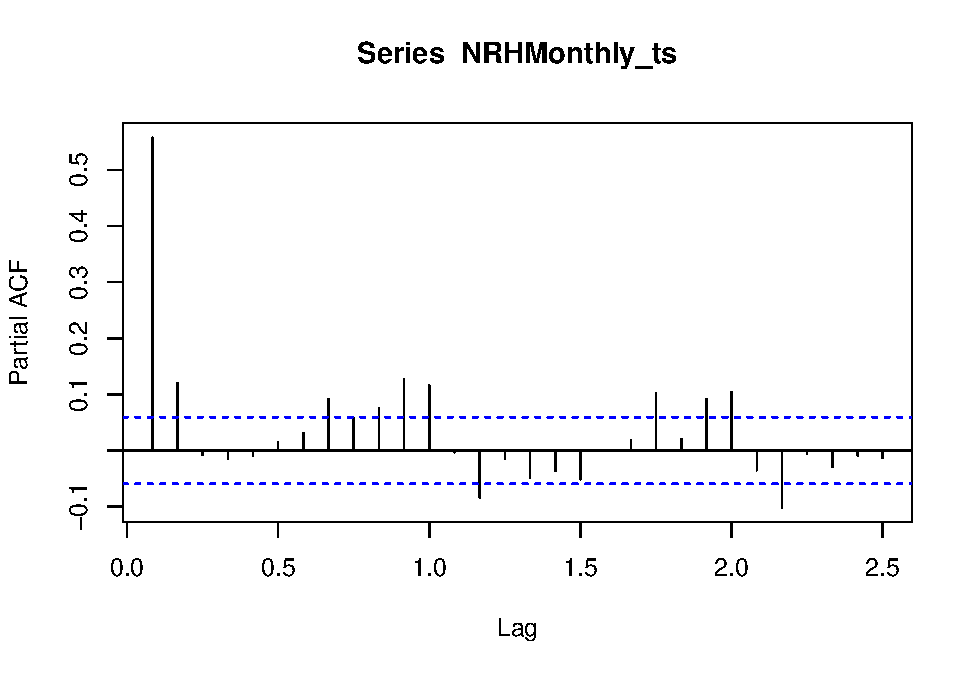
\includegraphics{Project_Template_files/figure-latex/unnamed-chunk-6-6.pdf}

\begin{Shaded}
\begin{Highlighting}[]
\CommentTok{# run the arima function and search for best fit}
\KeywordTok{auto.arima}\NormalTok{(NRHMonthly_ts, }\DataTypeTok{trace =} \OtherTok{TRUE}\NormalTok{)}
\end{Highlighting}
\end{Shaded}

\begin{verbatim}
## 
##  Fitting models using approximations to speed things up...
## 
##  ARIMA(2,1,2)(1,0,1)[12] with drift         : Inf
##  ARIMA(0,1,0)            with drift         : 19302.7
##  ARIMA(1,1,0)(1,0,0)[12] with drift         : 19168.62
##  ARIMA(0,1,1)(0,0,1)[12] with drift         : 19120.96
##  ARIMA(0,1,0)                               : 19300.7
##  ARIMA(0,1,1)            with drift         : 19146.2
##  ARIMA(0,1,1)(1,0,1)[12] with drift         : Inf
##  ARIMA(0,1,1)(0,0,2)[12] with drift         : 19094.06
##  ARIMA(0,1,1)(1,0,2)[12] with drift         : Inf
##  ARIMA(0,1,0)(0,0,2)[12] with drift         : 19284.84
##  ARIMA(1,1,1)(0,0,2)[12] with drift         : Inf
##  ARIMA(0,1,2)(0,0,2)[12] with drift         : 19052.68
##  ARIMA(0,1,2)(0,0,1)[12] with drift         : 19068.11
##  ARIMA(0,1,2)(1,0,2)[12] with drift         : Inf
##  ARIMA(0,1,2)(1,0,1)[12] with drift         : Inf
##  ARIMA(1,1,2)(0,0,2)[12] with drift         : Inf
##  ARIMA(0,1,3)(0,0,2)[12] with drift         : Inf
##  ARIMA(1,1,3)(0,0,2)[12] with drift         : Inf
##  ARIMA(0,1,2)(0,0,2)[12]                    : 19050.72
##  ARIMA(0,1,2)(0,0,1)[12]                    : 19066.22
##  ARIMA(0,1,2)(1,0,2)[12]                    : Inf
##  ARIMA(0,1,2)(1,0,1)[12]                    : Inf
##  ARIMA(0,1,1)(0,0,2)[12]                    : 19092.05
##  ARIMA(1,1,2)(0,0,2)[12]                    : 18972.02
##  ARIMA(1,1,2)(0,0,1)[12]                    : 18988.33
##  ARIMA(1,1,2)(1,0,2)[12]                    : Inf
##  ARIMA(1,1,2)(1,0,1)[12]                    : Inf
##  ARIMA(1,1,1)(0,0,2)[12]                    : 18982.4
##  ARIMA(2,1,2)(0,0,2)[12]                    : Inf
##  ARIMA(1,1,3)(0,0,2)[12]                    : Inf
##  ARIMA(0,1,3)(0,0,2)[12]                    : 18994.1
##  ARIMA(2,1,1)(0,0,2)[12]                    : Inf
##  ARIMA(2,1,3)(0,0,2)[12]                    : Inf
## 
##  Now re-fitting the best model(s) without approximations...
## 
##  ARIMA(1,1,2)(0,0,2)[12]                    : Inf
##  ARIMA(1,1,1)(0,0,2)[12]                    : 18997.57
## 
##  Best model: ARIMA(1,1,1)(0,0,2)[12]
\end{verbatim}

\begin{verbatim}
## Series: NRHMonthly_ts 
## ARIMA(1,1,1)(0,0,2)[12] 
## 
## Coefficients:
##          ar1      ma1    sma1    sma2
##       0.4935  -0.9892  0.1054  0.1108
## s.e.  0.0274   0.0053  0.0318  0.0289
## 
## sigma^2 estimated as 2053595:  log likelihood=-9493.76
## AIC=18997.51   AICc=18997.57   BIC=19022.5
\end{verbatim}

\begin{Shaded}
\begin{Highlighting}[]
\CommentTok{# create an object that defines the best fit model}
\NormalTok{NRHfit <-}\StringTok{ }\KeywordTok{arima}\NormalTok{(NRHMonthly_ts, }\KeywordTok{c}\NormalTok{(}\DecValTok{1}\NormalTok{, }\DecValTok{1}\NormalTok{, }\DecValTok{1}\NormalTok{),}\DataTypeTok{seasonal =} \KeywordTok{list}\NormalTok{(}\DataTypeTok{order =} \KeywordTok{c}\NormalTok{(}\DecValTok{0}\NormalTok{, }\DecValTok{0}\NormalTok{, }\DecValTok{2}\NormalTok{), }\DataTypeTok{period =} \DecValTok{12}\NormalTok{))}

\CommentTok{# make a prediction into the future}
\NormalTok{NRHprediction <-}\StringTok{ }\KeywordTok{predict}\NormalTok{(NRHfit, }\DataTypeTok{n.ahead =} \DecValTok{10}\OperatorTok{*}\DecValTok{12}\NormalTok{)}

\CommentTok{# plot future predictions}
\KeywordTok{ts.plot}\NormalTok{(NRHMonthly_ts, NRHprediction}\OperatorTok{$}\NormalTok{pred, }\DataTypeTok{lty =} \KeywordTok{c}\NormalTok{(}\DecValTok{1}\NormalTok{, }\DecValTok{3}\NormalTok{))}
\end{Highlighting}
\end{Shaded}

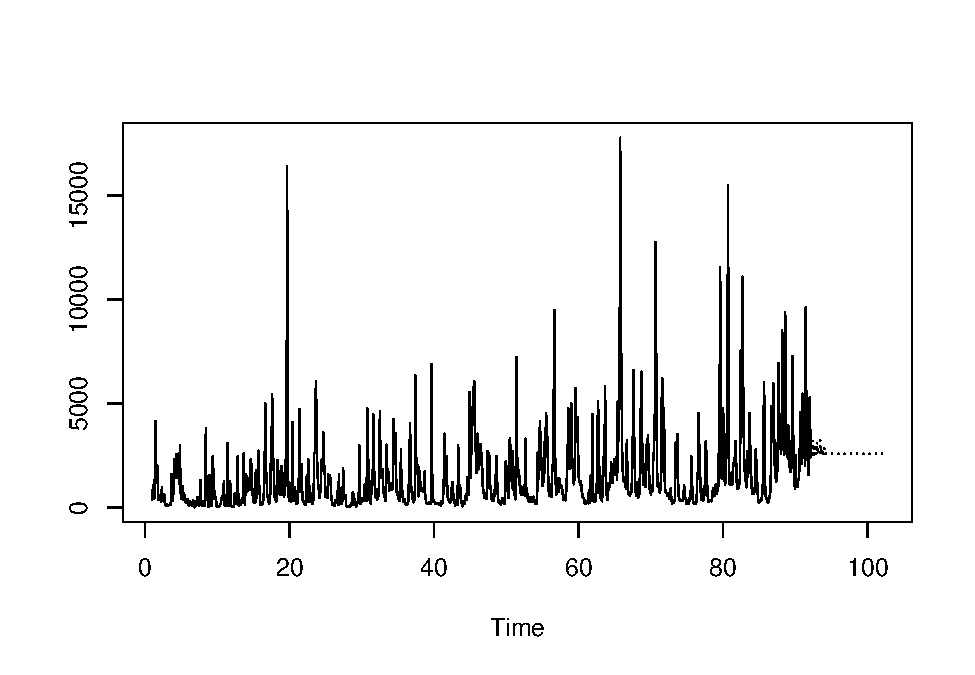
\includegraphics{Project_Template_files/figure-latex/unnamed-chunk-6-7.pdf}

\begin{Shaded}
\begin{Highlighting}[]
\CommentTok{########################### Nitrogen Analysis ############################}
\CommentTok{# Generate monthly values from March 2004 to September 2014}
\NormalTok{NRHNitrogenlp <-}\StringTok{ }\KeywordTok{as.data.frame}\NormalTok{(}\KeywordTok{approx}\NormalTok{(NRHNitrogen, }\DataTypeTok{n =} \DecValTok{128}\NormalTok{, }\DataTypeTok{method =} \StringTok{"linear"}\NormalTok{))}
\NormalTok{NRHNitrogenlp}\OperatorTok{$}\NormalTok{x <-}\StringTok{ }\KeywordTok{as.Date}\NormalTok{(NRHNitrogenlp}\OperatorTok{$}\NormalTok{x, }\DataTypeTok{origin =} \StringTok{"1970-01-01"}\NormalTok{)}
\KeywordTok{names}\NormalTok{(NRHNitrogenlp) <-}\StringTok{ }\KeywordTok{c}\NormalTok{(}\StringTok{"Date"}\NormalTok{, }\StringTok{"N"}\NormalTok{)}

\CommentTok{# Inspect interpolated values}
\NormalTok{NRHNinterpolated <-}
\StringTok{  }\KeywordTok{ggplot}\NormalTok{(NRHNitrogen, }\KeywordTok{aes}\NormalTok{(}\DataTypeTok{x =}\NormalTok{ sample_dt, }\DataTypeTok{y =}\NormalTok{ result_va)) }\OperatorTok{+}
\StringTok{  }\KeywordTok{geom_point}\NormalTok{() }\OperatorTok{+}
\StringTok{  }\KeywordTok{geom_line}\NormalTok{() }\OperatorTok{+}
\StringTok{  }\KeywordTok{geom_point}\NormalTok{(}\DataTypeTok{data =}\NormalTok{ NRHNitrogenlp, }\KeywordTok{aes}\NormalTok{(}\DataTypeTok{x =}\NormalTok{ Date, }\DataTypeTok{y =}\NormalTok{ N), }\DataTypeTok{color =} \StringTok{"#c13d75ff"}\NormalTok{)}
\KeywordTok{print}\NormalTok{(NRHNinterpolated)}
\end{Highlighting}
\end{Shaded}

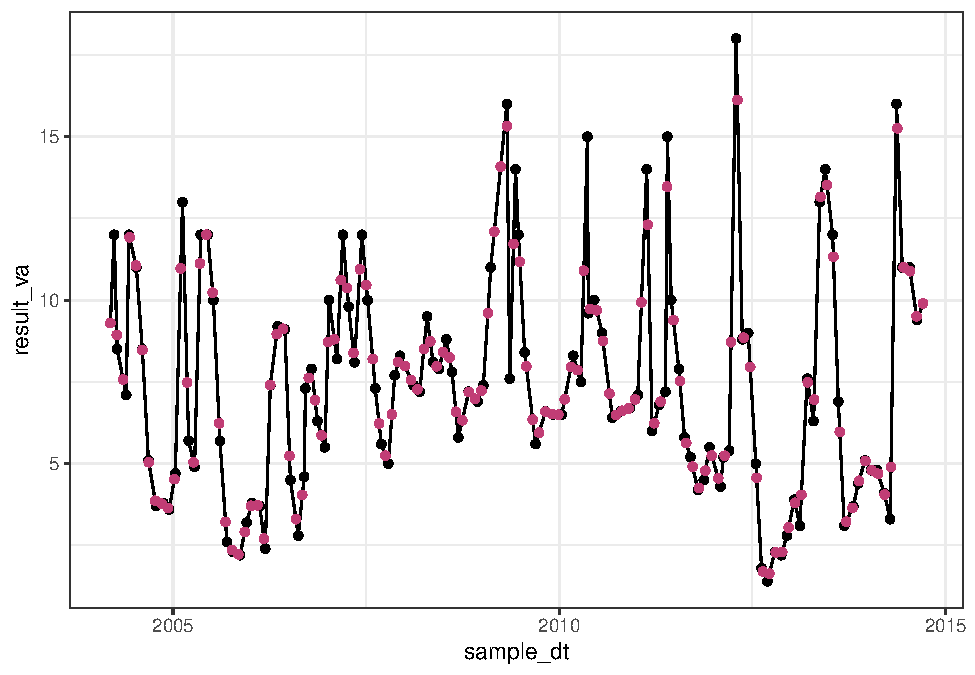
\includegraphics{Project_Template_files/figure-latex/unnamed-chunk-6-8.pdf}

\begin{Shaded}
\begin{Highlighting}[]
\CommentTok{# Generate time series (smk.test needs ts, not data.frame)}
\NormalTok{NRHNtimeseries <-}\StringTok{ }\KeywordTok{ts}\NormalTok{(NRHNitrogenlp}\OperatorTok{$}\NormalTok{N, }\DataTypeTok{frequency =} \DecValTok{12}\NormalTok{,}
                     \DataTypeTok{start =} \KeywordTok{c}\NormalTok{(}\DecValTok{2004}\NormalTok{, }\DecValTok{3}\NormalTok{, }\DecValTok{11}\NormalTok{), }\DataTypeTok{end =} \KeywordTok{c}\NormalTok{(}\DecValTok{2014}\NormalTok{, }\DecValTok{9}\NormalTok{, }\DecValTok{16}\NormalTok{))}
\CommentTok{# Run SMK test}
\NormalTok{NRHNtrend <-}\StringTok{ }\KeywordTok{smk.test}\NormalTok{(NRHNtimeseries)}

\CommentTok{# Inspect results}
\NormalTok{NRHNtrend}
\end{Highlighting}
\end{Shaded}

\begin{verbatim}
## 
##  Seasonal Mann-Kendall trend test (Hirsch-Slack test)
## 
## data:  NRHNtimeseries
## z = -0.63996, p-value = 0.5222
## alternative hypothesis: true S is not equal to 0
## sample estimates:
##    S varS 
##  -28 1780
\end{verbatim}

\begin{Shaded}
\begin{Highlighting}[]
\KeywordTok{summary}\NormalTok{(NRHNtrend)}
\end{Highlighting}
\end{Shaded}

\begin{verbatim}
## 
##  Seasonal Mann-Kendall trend test (Hirsch-Slack test)
## 
## data: NRHNtimeseries
## alternative hypothesis: two.sided
## 
## Statistics for individual seasons
## 
## H0
##                      S varS    tau      z Pr(>|z|)  
## Season 1:   S = 0  -13  125 -0.289 -1.073  0.28313  
## Season 2:   S = 0  -13  125 -0.289 -1.073  0.28313  
## Season 3:   S = 0   -9  165 -0.164 -0.623  0.53342  
## Season 4:   S = 0  -11  165 -0.200 -0.778  0.43627  
## Season 5:   S = 0   -9  165 -0.164 -0.623  0.53342  
## Season 6:   S = 0   11  165  0.200  0.778  0.43627  
## Season 7:   S = 0    3  165  0.055  0.156  0.87627  
## Season 8:   S = 0   13  165  0.236  0.934  0.35020  
## Season 9:   S = 0   17  165  0.309  1.246  0.21291  
## Season 10:   S = 0  -7  125 -0.156 -0.537  0.59151  
## Season 11:   S = 0  -5  125 -0.111 -0.358  0.72051  
## Season 12:   S = 0  -5  125 -0.111 -0.358  0.72051  
## ---
## Signif. codes:  0 '***' 0.001 '**' 0.01 '*' 0.05 '.' 0.1 ' ' 1
\end{verbatim}

\begin{Shaded}
\begin{Highlighting}[]
\CommentTok{########################### Phosphorus Analysis ############################}
\CommentTok{# Generate monthly values from March 2004 to September 2014}
\NormalTok{NRHPhosphoruslp <-}\StringTok{ }\KeywordTok{as.data.frame}\NormalTok{(}\KeywordTok{approx}\NormalTok{(NRHPhosphorus, }\DataTypeTok{n =} \DecValTok{128}\NormalTok{, }\DataTypeTok{method =} \StringTok{"linear"}\NormalTok{))}
\NormalTok{NRHPhosphoruslp}\OperatorTok{$}\NormalTok{x <-}\StringTok{ }\KeywordTok{as.Date}\NormalTok{(NRHPhosphoruslp}\OperatorTok{$}\NormalTok{x, }\DataTypeTok{origin =} \StringTok{"1970-01-01"}\NormalTok{)}
\KeywordTok{names}\NormalTok{(NRHPhosphoruslp) <-}\StringTok{ }\KeywordTok{c}\NormalTok{(}\StringTok{"Date"}\NormalTok{, }\StringTok{"P"}\NormalTok{)}

\CommentTok{# Inspect interpolated values}
\NormalTok{NRHPinterpolated <-}
\StringTok{  }\KeywordTok{ggplot}\NormalTok{(NRHPhosphorus, }\KeywordTok{aes}\NormalTok{(}\DataTypeTok{x =}\NormalTok{ sample_dt, }\DataTypeTok{y =}\NormalTok{ result_va)) }\OperatorTok{+}
\StringTok{  }\KeywordTok{geom_point}\NormalTok{() }\OperatorTok{+}
\StringTok{  }\KeywordTok{geom_line}\NormalTok{() }\OperatorTok{+}
\StringTok{  }\KeywordTok{geom_point}\NormalTok{(}\DataTypeTok{data =}\NormalTok{ NRHPhosphoruslp, }\KeywordTok{aes}\NormalTok{(}\DataTypeTok{x =}\NormalTok{ Date, }\DataTypeTok{y =}\NormalTok{ P), }\DataTypeTok{color =} \StringTok{"#c13d75ff"}\NormalTok{)}
\KeywordTok{print}\NormalTok{(NRHPinterpolated)}
\end{Highlighting}
\end{Shaded}

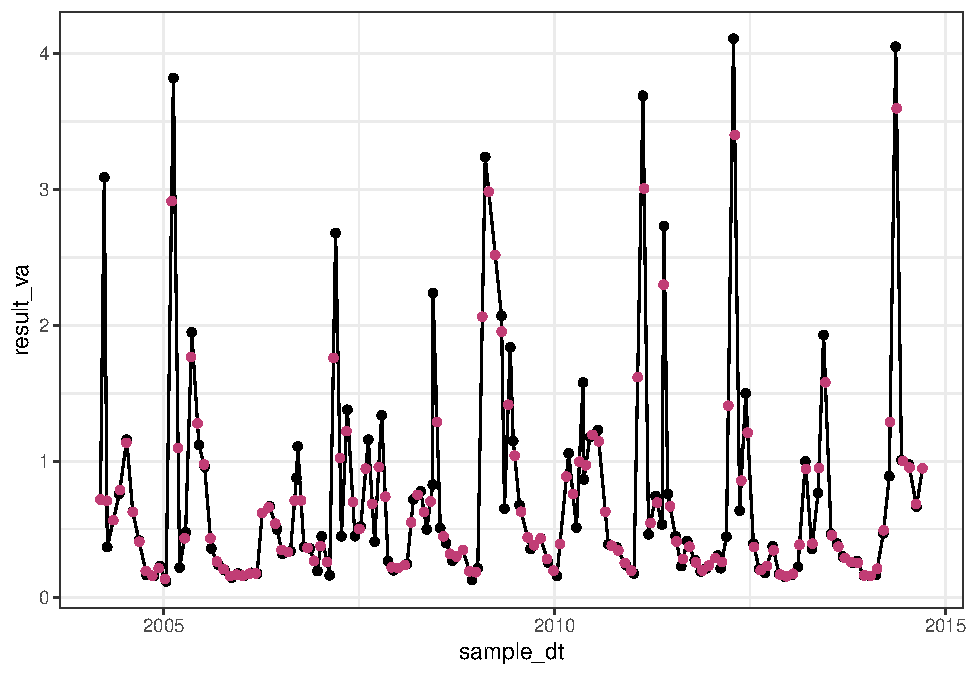
\includegraphics{Project_Template_files/figure-latex/unnamed-chunk-6-9.pdf}

\begin{Shaded}
\begin{Highlighting}[]
\CommentTok{# Generate time series (smk.test needs ts, not data.frame)}
\NormalTok{NRHPtimeseries <-}\StringTok{ }\KeywordTok{ts}\NormalTok{(NRHPhosphoruslp}\OperatorTok{$}\NormalTok{P, }\DataTypeTok{frequency =} \DecValTok{12}\NormalTok{,}
                     \DataTypeTok{start =} \KeywordTok{c}\NormalTok{(}\DecValTok{2004}\NormalTok{, }\DecValTok{3}\NormalTok{, }\DecValTok{11}\NormalTok{), }\DataTypeTok{end =} \KeywordTok{c}\NormalTok{(}\DecValTok{2014}\NormalTok{, }\DecValTok{9}\NormalTok{, }\DecValTok{16}\NormalTok{))}
\CommentTok{# Run SMK test}
\NormalTok{NRHPtrend <-}\StringTok{ }\KeywordTok{smk.test}\NormalTok{(NRHPtimeseries)}

\CommentTok{# Inspect results}
\NormalTok{NRHPtrend}
\end{Highlighting}
\end{Shaded}

\begin{verbatim}
## 
##  Seasonal Mann-Kendall trend test (Hirsch-Slack test)
## 
## data:  NRHPtimeseries
## z = 0.82958, p-value = 0.4068
## alternative hypothesis: true S is not equal to 0
## sample estimates:
##    S varS 
##   36 1780
\end{verbatim}

\begin{Shaded}
\begin{Highlighting}[]
\KeywordTok{summary}\NormalTok{(NRHPtrend)}
\end{Highlighting}
\end{Shaded}

\begin{verbatim}
## 
##  Seasonal Mann-Kendall trend test (Hirsch-Slack test)
## 
## data: NRHPtimeseries
## alternative hypothesis: two.sided
## 
## Statistics for individual seasons
## 
## H0
##                      S varS    tau      z Pr(>|z|)  
## Season 1:   S = 0    3  125  0.067  0.179 0.858028  
## Season 2:   S = 0  -15  125 -0.333 -1.252 0.210498  
## Season 3:   S = 0   -7  165 -0.127 -0.467 0.640429  
## Season 4:   S = 0    7  165  0.127  0.467 0.640429  
## Season 5:   S = 0    7  165  0.127  0.467 0.640429  
## Season 6:   S = 0   23  165  0.418  1.713 0.086768 .
## Season 7:   S = 0   15  165  0.273  1.090 0.275758  
## Season 8:   S = 0    7  165  0.127  0.467 0.640429  
## Season 9:   S = 0   -5  165 -0.091 -0.311 0.755497  
## Season 10:   S = 0  -1  125 -0.022  0.000 1.000000  
## Season 11:   S = 0  -1  125 -0.022  0.000 1.000000  
## Season 12:   S = 0   3  125  0.067  0.179 0.858028  
## ---
## Signif. codes:  0 '***' 0.001 '**' 0.01 '*' 0.05 '.' 0.1 ' ' 1
\end{verbatim}

\begin{Shaded}
\begin{Highlighting}[]
\CommentTok{# 06934500 Missouri River at Hermann, MO }

\CommentTok{########################### Discharge Analysis ############################}

\NormalTok{MRHRegressionPlot <-}\StringTok{ }
\StringTok{  }\KeywordTok{ggplot}\NormalTok{(MRHDischarge, }\KeywordTok{aes}\NormalTok{(}\DataTypeTok{x =}\NormalTok{ Date, }\DataTypeTok{y =}\NormalTok{ Discharge)) }\OperatorTok{+}
\StringTok{  }\KeywordTok{geom_line}\NormalTok{() }\OperatorTok{+}
\StringTok{  }\KeywordTok{geom_smooth}\NormalTok{(}\DataTypeTok{method =} \StringTok{"lm"}\NormalTok{, }\DataTypeTok{se =} \OtherTok{FALSE}\NormalTok{, }\DataTypeTok{color =} \StringTok{"#c13d75ff"}\NormalTok{) }\OperatorTok{+}
\StringTok{  }\KeywordTok{labs}\NormalTok{(}\DataTypeTok{x =} \StringTok{""}\NormalTok{, }\DataTypeTok{y =} \KeywordTok{expression}\NormalTok{(}\StringTok{"Discharge (ft"}\OperatorTok{^}\DecValTok{3}\OperatorTok{*}\StringTok{"/s)"}\NormalTok{)) }\OperatorTok{+}\StringTok{ }
\StringTok{  }\KeywordTok{theme}\NormalTok{(}\DataTypeTok{plot.title =} \KeywordTok{element_text}\NormalTok{(}\DataTypeTok{margin =} \KeywordTok{margin}\NormalTok{(}\DataTypeTok{b =} \DecValTok{-10}\NormalTok{), }\DataTypeTok{size =} \DecValTok{12}\NormalTok{), }
        \DataTypeTok{axis.title.x =} \KeywordTok{element_blank}\NormalTok{())}
\KeywordTok{print}\NormalTok{(MRHRegressionPlot)}
\end{Highlighting}
\end{Shaded}

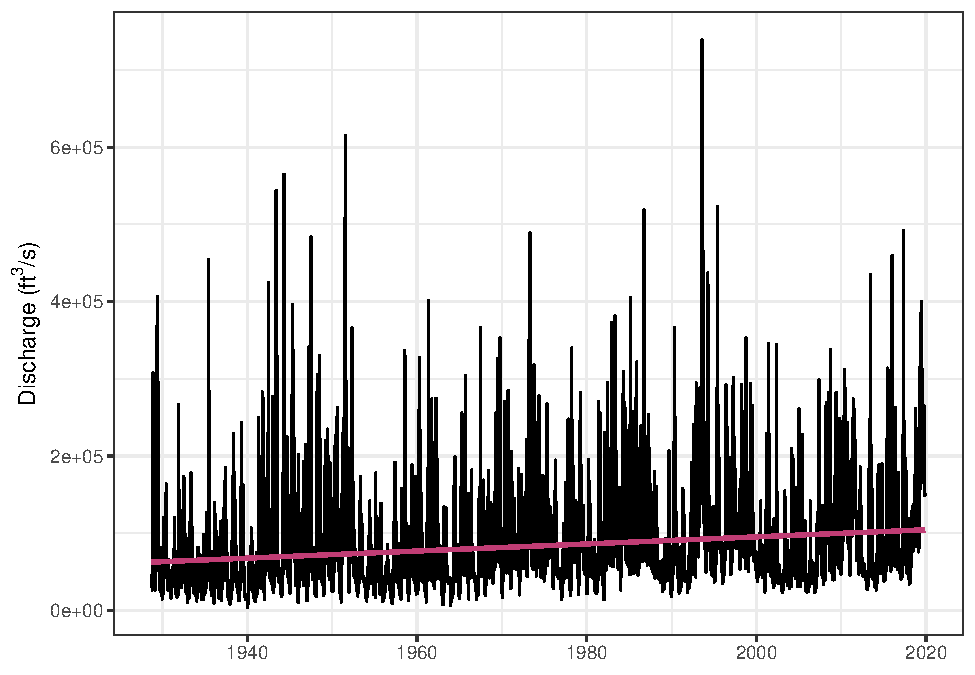
\includegraphics{Project_Template_files/figure-latex/unnamed-chunk-6-10.pdf}

\begin{Shaded}
\begin{Highlighting}[]
\NormalTok{MRHDischarge <-}\StringTok{ }\KeywordTok{na.omit}\NormalTok{(MRHDischarge)}
\NormalTok{MRH_ts <-}\StringTok{ }\KeywordTok{ts}\NormalTok{(MRHDischarge[[}\DecValTok{4}\NormalTok{]], }\DataTypeTok{frequency =} \DecValTok{365}\NormalTok{)}
\KeywordTok{table}\NormalTok{(}\KeywordTok{diff}\NormalTok{(MRHDischarge}\OperatorTok{$}\NormalTok{Date))}
\end{Highlighting}
\end{Shaded}

\begin{verbatim}
## 
##     1     3 
## 33276     1
\end{verbatim}

\begin{Shaded}
\begin{Highlighting}[]
\CommentTok{# Generate the decomposition}
\NormalTok{MRH_Decomposed <-}\StringTok{ }\KeywordTok{stl}\NormalTok{(MRH_ts, }\DataTypeTok{s.window =} \StringTok{"periodic"}\NormalTok{)}

\CommentTok{# Visualize the decomposed series. }
\KeywordTok{plot}\NormalTok{(MRH_Decomposed)}
\end{Highlighting}
\end{Shaded}

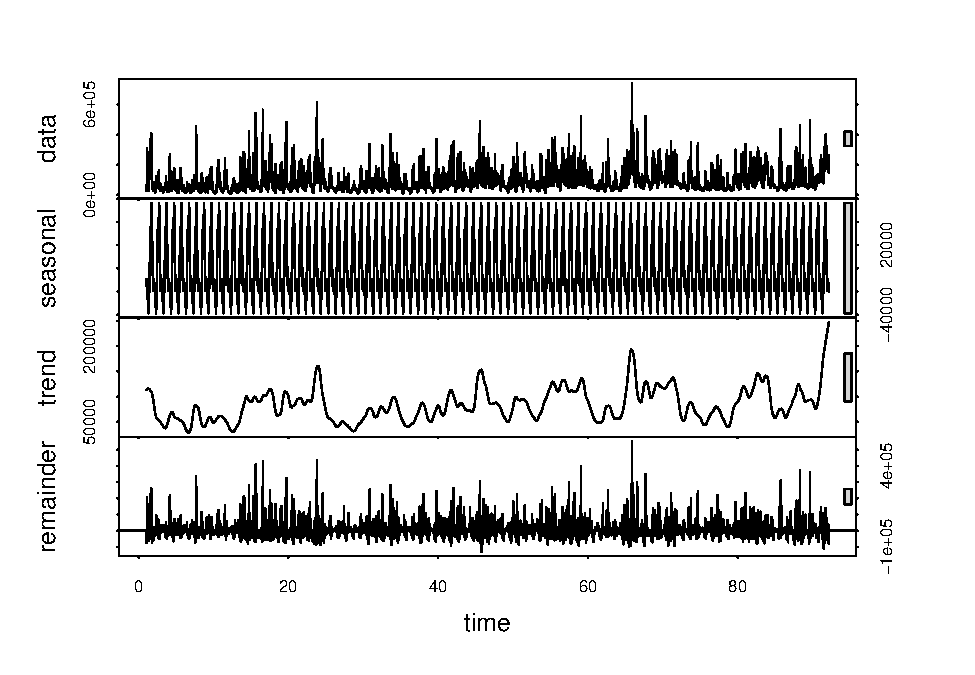
\includegraphics{Project_Template_files/figure-latex/unnamed-chunk-6-11.pdf}

\begin{Shaded}
\begin{Highlighting}[]
\CommentTok{# We can extract the components and turn them into data frames}
\NormalTok{MRH_Components <-}\StringTok{ }\KeywordTok{as.data.frame}\NormalTok{(MRH_Decomposed}\OperatorTok{$}\NormalTok{time.series[,}\DecValTok{1}\OperatorTok{:}\DecValTok{3}\NormalTok{])}
\NormalTok{MRH_Components <-}\StringTok{ }\KeywordTok{mutate}\NormalTok{(MRH_Components,}
                           \DataTypeTok{Observed =}\NormalTok{ MRHDischarge}\OperatorTok{$}\NormalTok{Discharge,     }
                           \DataTypeTok{Date =}\NormalTok{ MRHDischarge}\OperatorTok{$}\NormalTok{Date)}

\CommentTok{# Visualize how the trend maps onto the data}
\KeywordTok{ggplot}\NormalTok{(MRH_Components) }\OperatorTok{+}
\StringTok{  }\KeywordTok{geom_line}\NormalTok{(}\KeywordTok{aes}\NormalTok{(}\DataTypeTok{y =}\NormalTok{ Observed, }\DataTypeTok{x =}\NormalTok{ Date),  }\DataTypeTok{size =} \FloatTok{0.25}\NormalTok{) }\OperatorTok{+}
\StringTok{  }\KeywordTok{geom_line}\NormalTok{(}\KeywordTok{aes}\NormalTok{(}\DataTypeTok{y =}\NormalTok{ trend, }\DataTypeTok{x =}\NormalTok{ Date), }\DataTypeTok{color =} \StringTok{"#c13d75ff"}\NormalTok{) }\OperatorTok{+}
\StringTok{  }\KeywordTok{geom_hline}\NormalTok{(}\DataTypeTok{yintercept =} \DecValTok{0}\NormalTok{, }\DataTypeTok{lty =} \DecValTok{2}\NormalTok{) }\OperatorTok{+}
\StringTok{  }\KeywordTok{ylab}\NormalTok{(}\KeywordTok{expression}\NormalTok{(}\StringTok{"Discharge (ft"}\OperatorTok{^}\DecValTok{3}\OperatorTok{*}\StringTok{"/s)"}\NormalTok{))}
\end{Highlighting}
\end{Shaded}

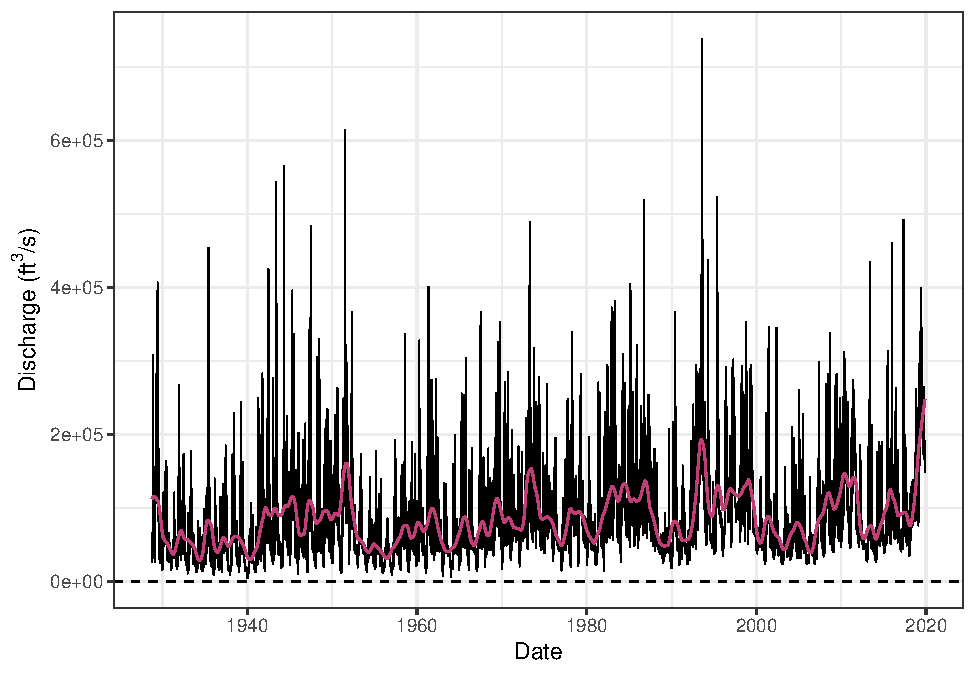
\includegraphics{Project_Template_files/figure-latex/unnamed-chunk-6-12.pdf}

\begin{Shaded}
\begin{Highlighting}[]
\CommentTok{# Visualize how the seasonal cycle maps onto the data}
\KeywordTok{ggplot}\NormalTok{(MRH_Components) }\OperatorTok{+}
\StringTok{  }\KeywordTok{geom_line}\NormalTok{(}\KeywordTok{aes}\NormalTok{(}\DataTypeTok{y =}\NormalTok{ Observed, }\DataTypeTok{x =}\NormalTok{ Date),  }\DataTypeTok{size =} \FloatTok{0.25}\NormalTok{) }\OperatorTok{+}
\StringTok{  }\KeywordTok{geom_line}\NormalTok{(}\KeywordTok{aes}\NormalTok{(}\DataTypeTok{y =}\NormalTok{ seasonal, }\DataTypeTok{x =}\NormalTok{ Date), }\DataTypeTok{color =} \StringTok{"#c13d75ff"}\NormalTok{) }\OperatorTok{+}
\StringTok{  }\KeywordTok{geom_hline}\NormalTok{(}\DataTypeTok{yintercept =} \DecValTok{0}\NormalTok{, }\DataTypeTok{lty =} \DecValTok{2}\NormalTok{) }\OperatorTok{+}
\StringTok{  }\KeywordTok{ylab}\NormalTok{(}\KeywordTok{expression}\NormalTok{(}\StringTok{"Discharge (ft"}\OperatorTok{^}\DecValTok{3}\OperatorTok{*}\StringTok{"/s)"}\NormalTok{))}
\end{Highlighting}
\end{Shaded}

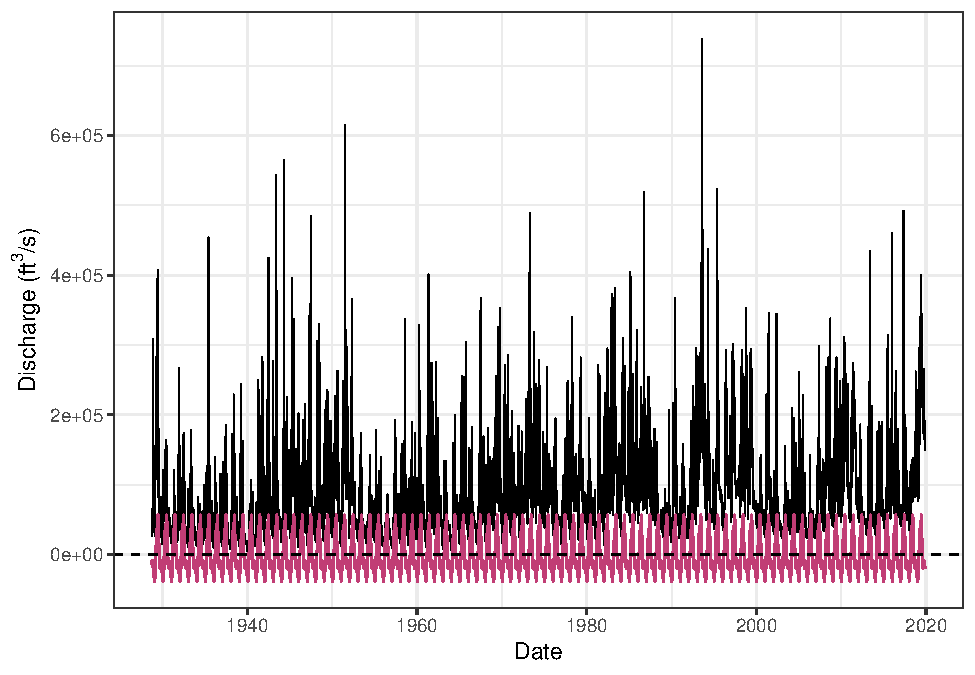
\includegraphics{Project_Template_files/figure-latex/unnamed-chunk-6-13.pdf}

\begin{Shaded}
\begin{Highlighting}[]
\NormalTok{MRHDischarge.Monthly <-}\StringTok{ }\NormalTok{MRHDischarge }\OperatorTok
\StringTok{  }\KeywordTok{mutate}\NormalTok{(}\DataTypeTok{Year =} \KeywordTok{year}\NormalTok{(Date),}
         \DataTypeTok{Month =} \KeywordTok{month}\NormalTok{(Date)) }\OperatorTok
\StringTok{  }\KeywordTok{group_by}\NormalTok{(Year, Month) }\OperatorTok
\StringTok{  }\KeywordTok{summarise}\NormalTok{(}\DataTypeTok{Discharge =} \KeywordTok{mean}\NormalTok{(Discharge))}
\NormalTok{MRHMonthly_ts <-}\StringTok{ }\KeywordTok{ts}\NormalTok{(MRHDischarge.Monthly[[}\DecValTok{3}\NormalTok{]], }\DataTypeTok{frequency =} \DecValTok{12}\NormalTok{)}
\KeywordTok{adf.test}\NormalTok{(MRHMonthly_ts, }\DataTypeTok{alternative =} \StringTok{"stationary"}\NormalTok{)}
\end{Highlighting}
\end{Shaded}

\begin{verbatim}
## Warning in adf.test(MRHMonthly_ts, alternative = "stationary"): p-value
## smaller than printed p-value
\end{verbatim}

\begin{verbatim}
## 
##  Augmented Dickey-Fuller Test
## 
## data:  MRHMonthly_ts
## Dickey-Fuller = -5.0751, Lag order = 10, p-value = 0.01
## alternative hypothesis: stationary
\end{verbatim}

\begin{Shaded}
\begin{Highlighting}[]
\KeywordTok{acf}\NormalTok{(MRHMonthly_ts)}
\end{Highlighting}
\end{Shaded}

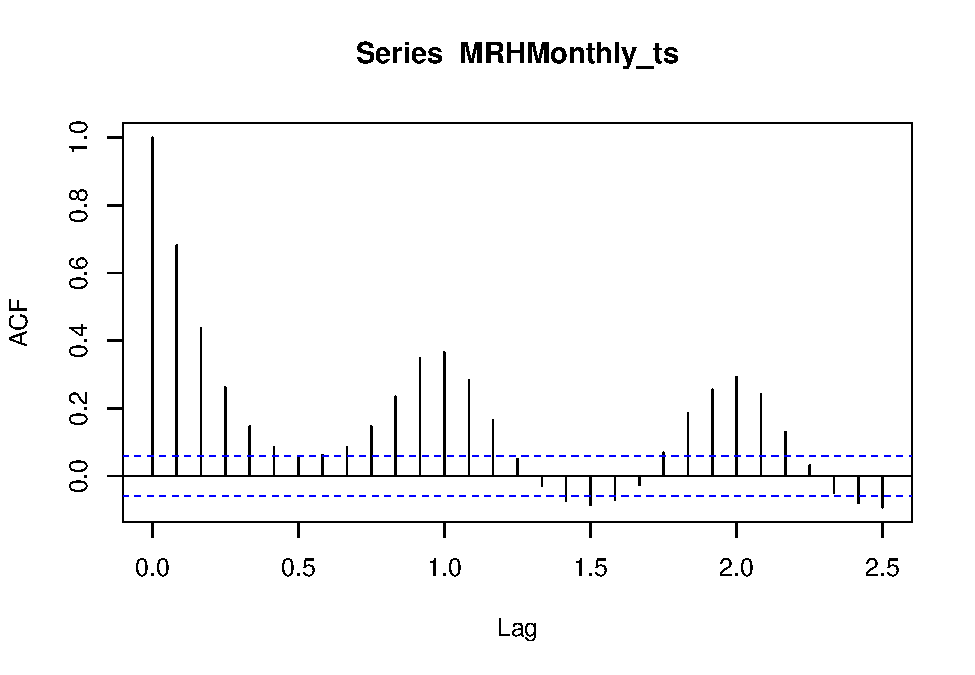
\includegraphics{Project_Template_files/figure-latex/unnamed-chunk-6-14.pdf}

\begin{Shaded}
\begin{Highlighting}[]
\KeywordTok{pacf}\NormalTok{(MRHMonthly_ts)}
\end{Highlighting}
\end{Shaded}

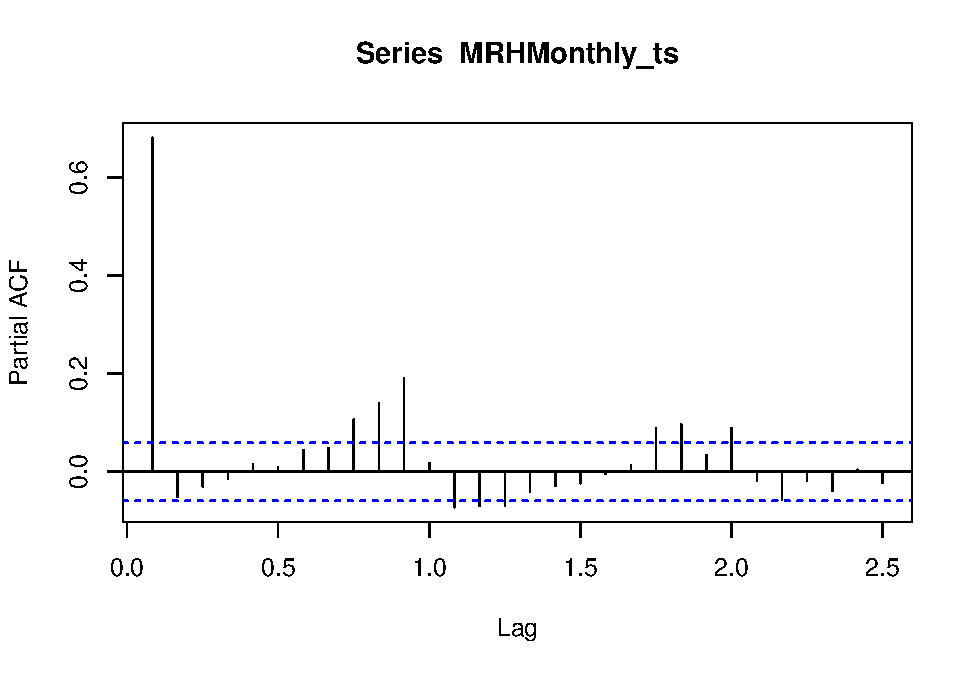
\includegraphics{Project_Template_files/figure-latex/unnamed-chunk-6-15.pdf}

\begin{Shaded}
\begin{Highlighting}[]
\CommentTok{# run the arima function and search for best fit}
\KeywordTok{auto.arima}\NormalTok{(MRHMonthly_ts, }\DataTypeTok{trace =} \OtherTok{TRUE}\NormalTok{)}
\end{Highlighting}
\end{Shaded}

\begin{verbatim}
## 
##  Fitting models using approximations to speed things up...
## 
##  ARIMA(2,1,2)(1,0,1)[12] with drift         : Inf
##  ARIMA(0,1,0)            with drift         : 26461.72
##  ARIMA(1,1,0)(1,0,0)[12] with drift         : 26386.98
##  ARIMA(0,1,1)(0,0,1)[12] with drift         : 26407.7
##  ARIMA(0,1,0)                               : 26459.72
##  ARIMA(1,1,0)            with drift         : 26445.3
##  ARIMA(1,1,0)(2,0,0)[12] with drift         : 26374.86
##  ARIMA(1,1,0)(2,0,1)[12] with drift         : Inf
##  ARIMA(1,1,0)(1,0,1)[12] with drift         : Inf
##  ARIMA(0,1,0)(2,0,0)[12] with drift         : 26410.1
##  ARIMA(2,1,0)(2,0,0)[12] with drift         : 26346.77
##  ARIMA(2,1,0)(1,0,0)[12] with drift         : 26366.23
##  ARIMA(2,1,0)(2,0,1)[12] with drift         : Inf
##  ARIMA(2,1,0)(1,0,1)[12] with drift         : Inf
##  ARIMA(3,1,0)(2,0,0)[12] with drift         : 26326.8
##  ARIMA(3,1,0)(1,0,0)[12] with drift         : 26350.81
##  ARIMA(3,1,0)(2,0,1)[12] with drift         : Inf
##  ARIMA(3,1,0)(1,0,1)[12] with drift         : Inf
##  ARIMA(4,1,0)(2,0,0)[12] with drift         : 26310.75
##  ARIMA(4,1,0)(1,0,0)[12] with drift         : 26332.4
##  ARIMA(4,1,0)(2,0,1)[12] with drift         : Inf
##  ARIMA(4,1,0)(1,0,1)[12] with drift         : Inf
##  ARIMA(5,1,0)(2,0,0)[12] with drift         : 26298.17
##  ARIMA(5,1,0)(1,0,0)[12] with drift         : 26319.67
##  ARIMA(5,1,0)(2,0,1)[12] with drift         : Inf
##  ARIMA(5,1,0)(1,0,1)[12] with drift         : Inf
##  ARIMA(5,1,1)(2,0,0)[12] with drift         : 26219.71
##  ARIMA(5,1,1)(1,0,0)[12] with drift         : 26224.97
##  ARIMA(5,1,1)(2,0,1)[12] with drift         : Inf
##  ARIMA(5,1,1)(1,0,1)[12] with drift         : Inf
##  ARIMA(4,1,1)(2,0,0)[12] with drift         : Inf
##  ARIMA(5,1,2)(2,0,0)[12] with drift         : Inf
##  ARIMA(4,1,2)(2,0,0)[12] with drift         : Inf
##  ARIMA(5,1,1)(2,0,0)[12]                    : 26219.03
##  ARIMA(5,1,1)(1,0,0)[12]                    : 26224.22
##  ARIMA(5,1,1)(2,0,1)[12]                    : Inf
##  ARIMA(5,1,1)(1,0,1)[12]                    : Inf
##  ARIMA(4,1,1)(2,0,0)[12]                    : Inf
##  ARIMA(5,1,0)(2,0,0)[12]                    : 26296.19
##  ARIMA(5,1,2)(2,0,0)[12]                    : Inf
##  ARIMA(4,1,0)(2,0,0)[12]                    : 26308.76
##  ARIMA(4,1,2)(2,0,0)[12]                    : 26212.54
##  ARIMA(4,1,2)(1,0,0)[12]                    : 26225.14
##  ARIMA(4,1,2)(2,0,1)[12]                    : Inf
##  ARIMA(4,1,2)(1,0,1)[12]                    : Inf
##  ARIMA(3,1,2)(2,0,0)[12]                    : Inf
##  ARIMA(4,1,3)(2,0,0)[12]                    : 26214.31
##  ARIMA(3,1,1)(2,0,0)[12]                    : 26212.12
##  ARIMA(3,1,1)(1,0,0)[12]                    : Inf
##  ARIMA(3,1,1)(2,0,1)[12]                    : Inf
##  ARIMA(3,1,1)(1,0,1)[12]                    : Inf
##  ARIMA(2,1,1)(2,0,0)[12]                    : Inf
##  ARIMA(3,1,0)(2,0,0)[12]                    : 26324.8
##  ARIMA(2,1,0)(2,0,0)[12]                    : 26344.76
##  ARIMA(2,1,2)(2,0,0)[12]                    : Inf
##  ARIMA(3,1,1)(2,0,0)[12] with drift         : 26212.76
## 
##  Now re-fitting the best model(s) without approximations...
## 
##  ARIMA(3,1,1)(2,0,0)[12]                    : Inf
##  ARIMA(4,1,2)(2,0,0)[12]                    : Inf
##  ARIMA(3,1,1)(2,0,0)[12] with drift         : Inf
##  ARIMA(4,1,3)(2,0,0)[12]                    : Inf
##  ARIMA(5,1,1)(2,0,0)[12]                    : Inf
##  ARIMA(5,1,1)(2,0,0)[12] with drift         : Inf
##  ARIMA(5,1,1)(1,0,0)[12]                    : Inf
##  ARIMA(5,1,1)(1,0,0)[12] with drift         : Inf
##  ARIMA(4,1,2)(1,0,0)[12]                    : Inf
##  ARIMA(5,1,0)(2,0,0)[12]                    : 26328.41
## 
##  Best model: ARIMA(5,1,0)(2,0,0)[12]
\end{verbatim}

\begin{verbatim}
## Series: MRHMonthly_ts 
## ARIMA(5,1,0)(2,0,0)[12] 
## 
## Coefficients:
##           ar1      ar2      ar3      ar4      ar5    sar1    sar2
##       -0.2814  -0.2466  -0.2048  -0.1659  -0.1196  0.1938  0.1783
## s.e.   0.0318   0.0319   0.0315   0.0309   0.0303  0.0312  0.0313
## 
## sigma^2 estimated as 1.677e+09:  log likelihood=-13156.14
## AIC=26328.28   AICc=26328.41   BIC=26368.26
\end{verbatim}

\begin{Shaded}
\begin{Highlighting}[]
\CommentTok{# create an object that defines the best fit model}
\NormalTok{MRHfit <-}\StringTok{ }\KeywordTok{arima}\NormalTok{(MRHMonthly_ts, }\KeywordTok{c}\NormalTok{(}\DecValTok{5}\NormalTok{, }\DecValTok{1}\NormalTok{, }\DecValTok{0}\NormalTok{), }\DataTypeTok{seasonal =} \KeywordTok{list}\NormalTok{(}\DataTypeTok{order =} \KeywordTok{c}\NormalTok{(}\DecValTok{2}\NormalTok{, }\DecValTok{0}\NormalTok{, }\DecValTok{0}\NormalTok{), }\DataTypeTok{period =} \DecValTok{12}\NormalTok{))}

\CommentTok{# make a prediction into the future}
\NormalTok{MRHprediction <-}\StringTok{ }\KeywordTok{predict}\NormalTok{(MRHfit, }\DataTypeTok{n.ahead =} \DecValTok{10}\OperatorTok{*}\DecValTok{12}\NormalTok{)}

\CommentTok{# plot future predictions}
\KeywordTok{ts.plot}\NormalTok{(MRHMonthly_ts, MRHprediction}\OperatorTok{$}\NormalTok{pred, }\DataTypeTok{lty =} \KeywordTok{c}\NormalTok{(}\DecValTok{1}\NormalTok{, }\DecValTok{3}\NormalTok{))}
\end{Highlighting}
\end{Shaded}

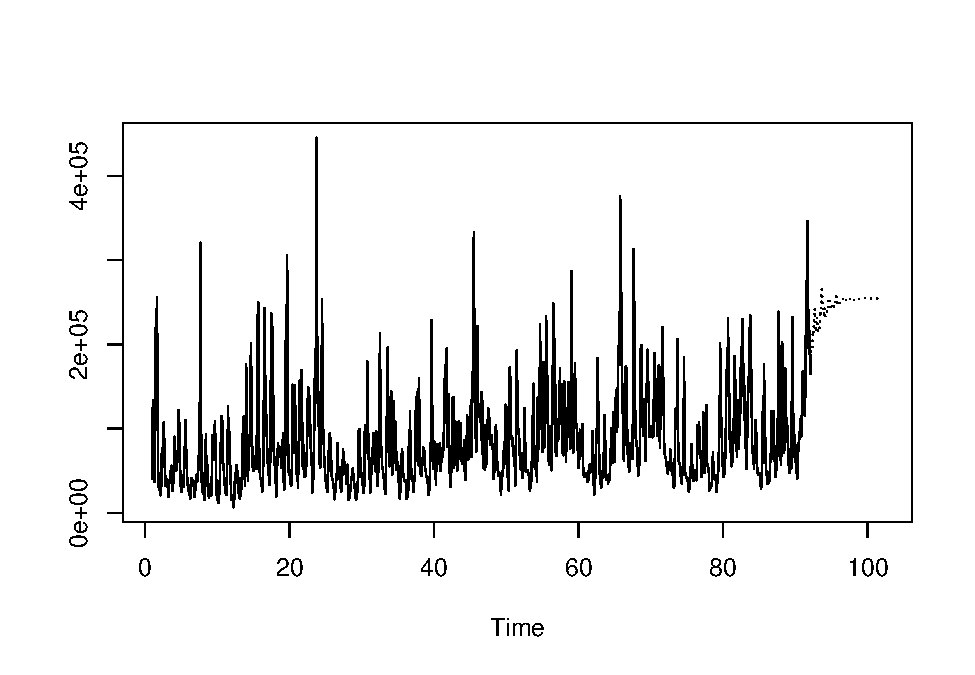
\includegraphics{Project_Template_files/figure-latex/unnamed-chunk-6-16.pdf}

\begin{Shaded}
\begin{Highlighting}[]
\CommentTok{########################### Nitrogen Analysis ############################}
\CommentTok{# Generate monthly values from July 1973 to August 2019}
\NormalTok{MRHNitrogenlp <-}\StringTok{ }\KeywordTok{as.data.frame}\NormalTok{(}\KeywordTok{approx}\NormalTok{(MRHNitrogen, }\DataTypeTok{n =} \DecValTok{556}\NormalTok{, }\DataTypeTok{method =} \StringTok{"linear"}\NormalTok{))}
\end{Highlighting}
\end{Shaded}

\begin{verbatim}
## Warning in regularize.values(x, y, ties, missing(ties)): collapsing to
## unique 'x' values
\end{verbatim}

\begin{Shaded}
\begin{Highlighting}[]
\NormalTok{MRHNitrogenlp}\OperatorTok{$}\NormalTok{x <-}\StringTok{ }\KeywordTok{as.Date}\NormalTok{(MRHNitrogenlp}\OperatorTok{$}\NormalTok{x, }\DataTypeTok{origin =} \StringTok{"1970-01-01"}\NormalTok{)}
\KeywordTok{names}\NormalTok{(MRHNitrogenlp) <-}\StringTok{ }\KeywordTok{c}\NormalTok{(}\StringTok{"Date"}\NormalTok{, }\StringTok{"N"}\NormalTok{)}

\CommentTok{# Inspect interpolated values}
\NormalTok{MRHNinterpolated <-}
\StringTok{  }\KeywordTok{ggplot}\NormalTok{(MRHNitrogen, }\KeywordTok{aes}\NormalTok{(}\DataTypeTok{x =}\NormalTok{ sample_dt, }\DataTypeTok{y =}\NormalTok{ result_va)) }\OperatorTok{+}
\StringTok{  }\KeywordTok{geom_point}\NormalTok{() }\OperatorTok{+}
\StringTok{  }\KeywordTok{geom_line}\NormalTok{() }\OperatorTok{+}
\StringTok{  }\KeywordTok{geom_point}\NormalTok{(}\DataTypeTok{data =}\NormalTok{ MRHNitrogenlp, }\KeywordTok{aes}\NormalTok{(}\DataTypeTok{x =}\NormalTok{ Date, }\DataTypeTok{y =}\NormalTok{ N), }\DataTypeTok{color =} \StringTok{"#c13d75ff"}\NormalTok{)}
\KeywordTok{print}\NormalTok{(MRHNinterpolated)}
\end{Highlighting}
\end{Shaded}

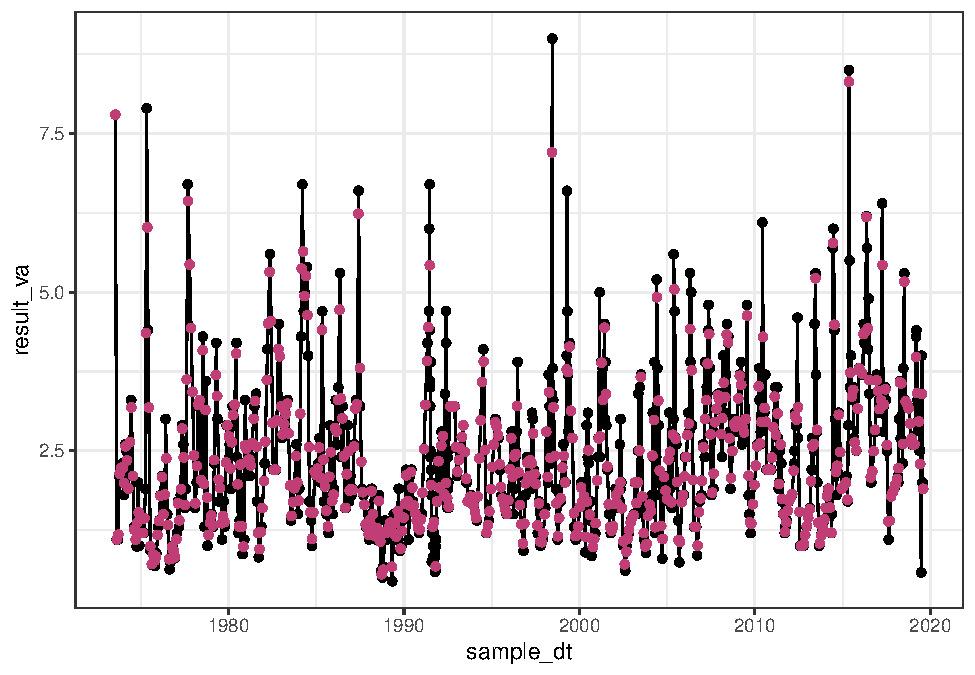
\includegraphics{Project_Template_files/figure-latex/unnamed-chunk-6-17.pdf}

\begin{Shaded}
\begin{Highlighting}[]
\CommentTok{# Generate time series (smk.test needs ts, not data.frame)}
\NormalTok{MRHNtimeseries <-}\StringTok{ }\KeywordTok{ts}\NormalTok{(MRHNitrogenlp}\OperatorTok{$}\NormalTok{N, }\DataTypeTok{frequency =} \DecValTok{12}\NormalTok{,}
                       \DataTypeTok{start =} \KeywordTok{c}\NormalTok{(}\DecValTok{1973}\NormalTok{, }\DecValTok{7}\NormalTok{, }\DecValTok{23}\NormalTok{), }\DataTypeTok{end =} \KeywordTok{c}\NormalTok{(}\DecValTok{2019}\NormalTok{, }\DecValTok{8}\NormalTok{, }\DecValTok{6}\NormalTok{))}
\CommentTok{# Run SMK test}
\NormalTok{MRHNtrend <-}\StringTok{ }\KeywordTok{smk.test}\NormalTok{(MRHNtimeseries)}

\CommentTok{# Inspect results}
\NormalTok{MRHNtrend}
\end{Highlighting}
\end{Shaded}

\begin{verbatim}
## 
##  Seasonal Mann-Kendall trend test (Hirsch-Slack test)
## 
## data:  MRHNtimeseries
## z = 3.8356, p-value = 0.0001253
## alternative hypothesis: true S is not equal to 0
## sample estimates:
##      S   varS 
##   1412 135330
\end{verbatim}

\begin{Shaded}
\begin{Highlighting}[]
\KeywordTok{summary}\NormalTok{(MRHNtrend)}
\end{Highlighting}
\end{Shaded}

\begin{verbatim}
## 
##  Seasonal Mann-Kendall trend test (Hirsch-Slack test)
## 
## data: MRHNtimeseries
## alternative hypothesis: two.sided
## 
## Statistics for individual seasons
## 
## H0
##                      S  varS    tau      z   Pr(>|z|)    
## Season 1:   S = 0   75 11155  0.072  0.701 0.48352569    
## Season 2:   S = 0   77 11155  0.074  0.720 0.47178391    
## Season 3:   S = 0   53 11155  0.051  0.492 0.62247625    
## Season 4:   S = 0  -54 11154 -0.052 -0.502 0.61578391    
## Season 5:   S = 0  -67 11155 -0.065 -0.625 0.53203799    
## Season 6:   S = 0   43 11155  0.042  0.398 0.69087907    
## Season 7:   S = 0  217 11891  0.201  1.981 0.04761169   *
## Season 8:   S = 0  539 11891  0.499  4.934 8.0685e-07 ***
## Season 9:   S = 0  378 11154  0.365  3.570 0.00035745 ***
## Season 10:   S = 0 103 11155  0.100  0.966 0.33416855    
## Season 11:   S = 0  37 11155  0.036  0.341 0.73321390    
## Season 12:   S = 0  11 11155  0.011  0.095 0.92456780    
## ---
## Signif. codes:  0 '***' 0.001 '**' 0.01 '*' 0.05 '.' 0.1 ' ' 1
\end{verbatim}

\begin{Shaded}
\begin{Highlighting}[]
\CommentTok{########################### Phosphorus Analysis ############################}
\CommentTok{# Generate monthly values from July 1969 to August 2019}
\NormalTok{MRHPhosphoruslp <-}\StringTok{ }\KeywordTok{as.data.frame}\NormalTok{(}\KeywordTok{approx}\NormalTok{(MRHPhosphorus, }\DataTypeTok{n =} \DecValTok{604}\NormalTok{, }\DataTypeTok{method =} \StringTok{"linear"}\NormalTok{))}
\end{Highlighting}
\end{Shaded}

\begin{verbatim}
## Warning in regularize.values(x, y, ties, missing(ties)): collapsing to
## unique 'x' values
\end{verbatim}

\begin{Shaded}
\begin{Highlighting}[]
\NormalTok{MRHPhosphoruslp}\OperatorTok{$}\NormalTok{x <-}\StringTok{ }\KeywordTok{as.Date}\NormalTok{(MRHPhosphoruslp}\OperatorTok{$}\NormalTok{x, }\DataTypeTok{origin =} \StringTok{"1970-01-01"}\NormalTok{)}
\KeywordTok{names}\NormalTok{(MRHPhosphoruslp) <-}\StringTok{ }\KeywordTok{c}\NormalTok{(}\StringTok{"Date"}\NormalTok{, }\StringTok{"P"}\NormalTok{)}

\CommentTok{# Inspect interpolated values}
\NormalTok{MRHPinterpolated <-}
\StringTok{  }\KeywordTok{ggplot}\NormalTok{(MRHPhosphorus, }\KeywordTok{aes}\NormalTok{(}\DataTypeTok{x =}\NormalTok{ sample_dt, }\DataTypeTok{y =}\NormalTok{ result_va)) }\OperatorTok{+}
\StringTok{  }\KeywordTok{geom_point}\NormalTok{() }\OperatorTok{+}
\StringTok{  }\KeywordTok{geom_line}\NormalTok{() }\OperatorTok{+}
\StringTok{  }\KeywordTok{geom_point}\NormalTok{(}\DataTypeTok{data =}\NormalTok{ MRHPhosphoruslp, }\KeywordTok{aes}\NormalTok{(}\DataTypeTok{x =}\NormalTok{ Date, }\DataTypeTok{y =}\NormalTok{ P), }\DataTypeTok{color =} \StringTok{"#c13d75ff"}\NormalTok{)}
\KeywordTok{print}\NormalTok{(MRHPinterpolated)}
\end{Highlighting}
\end{Shaded}

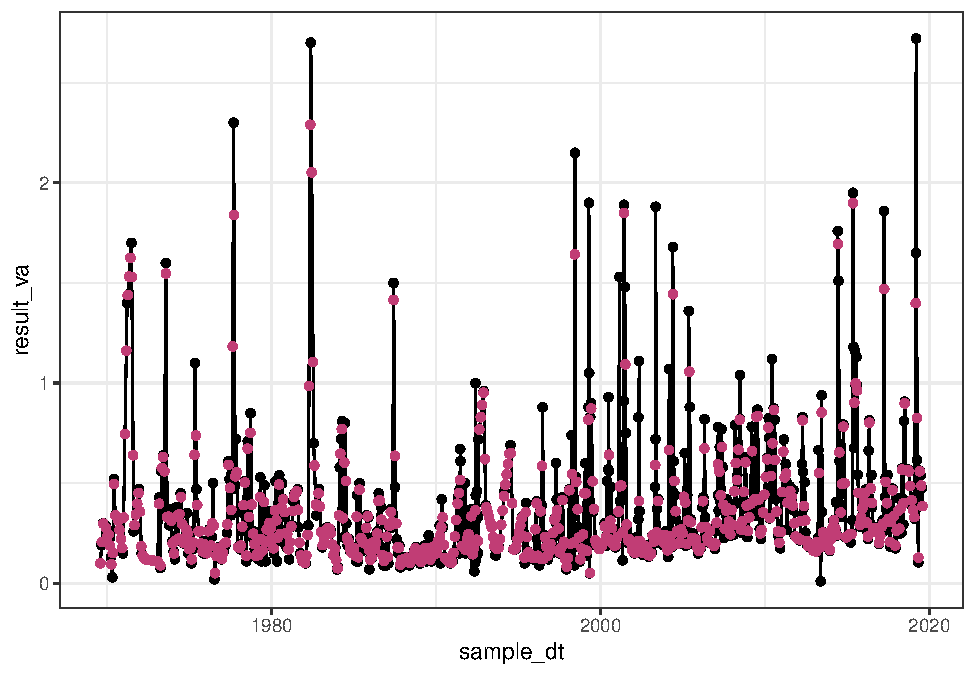
\includegraphics{Project_Template_files/figure-latex/unnamed-chunk-6-18.pdf}

\begin{Shaded}
\begin{Highlighting}[]
\CommentTok{# Generate time series (smk.test needs ts, not data.frame)}
\NormalTok{MRHPtimeseries <-}\StringTok{ }\KeywordTok{ts}\NormalTok{(MRHPhosphoruslp}\OperatorTok{$}\NormalTok{P, }\DataTypeTok{frequency =} \DecValTok{12}\NormalTok{,}
                       \DataTypeTok{start =} \KeywordTok{c}\NormalTok{(}\DecValTok{1969}\NormalTok{, }\DecValTok{7}\NormalTok{, }\DecValTok{31}\NormalTok{), }\DataTypeTok{end =} \KeywordTok{c}\NormalTok{(}\DecValTok{2019}\NormalTok{, }\DecValTok{8}\NormalTok{, }\DecValTok{6}\NormalTok{))}
\CommentTok{# Run SMK test}
\NormalTok{MRHPtrend <-}\StringTok{ }\KeywordTok{smk.test}\NormalTok{(MRHPtimeseries)}

\CommentTok{# Inspect results}
\NormalTok{MRHPtrend}
\end{Highlighting}
\end{Shaded}

\begin{verbatim}
## 
##  Seasonal Mann-Kendall trend test (Hirsch-Slack test)
## 
## data:  MRHPtimeseries
## z = 6.391, p-value = 1.648e-10
## alternative hypothesis: true S is not equal to 0
## sample estimates:
##        S     varS 
##   2661.0 173232.3
\end{verbatim}

\begin{Shaded}
\begin{Highlighting}[]
\KeywordTok{summary}\NormalTok{(MRHPtrend)}
\end{Highlighting}
\end{Shaded}

\begin{verbatim}
## 
##  Seasonal Mann-Kendall trend test (Hirsch-Slack test)
## 
## data: MRHPtimeseries
## alternative hypothesis: two.sided
## 
## Statistics for individual seasons
## 
## H0
##                      S    varS    tau      z  Pr(>|z|)   
## Season 1:   S = 0  371 14291.7  0.303  3.095 0.0019681 **
## Season 2:   S = 0  189 14291.7  0.154  1.573 0.1158130   
## Season 3:   S = 0  193 14291.7  0.158  1.606 0.1082623   
## Season 4:   S = 0   85 14291.7  0.069  0.703 0.4822751   
## Season 5:   S = 0  -35 14291.7 -0.029 -0.284 0.7760999   
## Season 6:   S = 0   87 14291.7  0.071  0.719 0.4719082   
## Season 7:   S = 0  181 15158.3  0.142  1.462 0.1437418   
## Season 8:   S = 0  405 15158.3  0.318  3.281 0.0010330 **
## Season 9:   S = 0  249 14291.7  0.203  2.074 0.0380343  *
## Season 10:   S = 0 283 14291.7  0.231  2.359 0.0183297  *
## Season 11:   S = 0 270 14290.7  0.220  2.250 0.0244346  *
## Season 12:   S = 0 383 14291.7  0.313  3.195 0.0013965 **
## ---
## Signif. codes:  0 '***' 0.001 '**' 0.01 '*' 0.05 '.' 0.1 ' ' 1
\end{verbatim}

\begin{Shaded}
\begin{Highlighting}[]
\CommentTok{# 06856600 REPUBLICAN R AT CLAY CENTER, KS}

\CommentTok{########################### Discharge Analysis ############################}
\NormalTok{RRCCRegressionPlot <-}\StringTok{ }
\StringTok{  }\KeywordTok{ggplot}\NormalTok{(RRCCDischarge, }\KeywordTok{aes}\NormalTok{(}\DataTypeTok{x =}\NormalTok{ Date, }\DataTypeTok{y =}\NormalTok{ Discharge)) }\OperatorTok{+}
\StringTok{  }\KeywordTok{geom_line}\NormalTok{() }\OperatorTok{+}
\StringTok{  }\KeywordTok{geom_smooth}\NormalTok{(}\DataTypeTok{method =} \StringTok{"lm"}\NormalTok{, }\DataTypeTok{se =} \OtherTok{FALSE}\NormalTok{, }\DataTypeTok{color =} \StringTok{"#c13d75ff"}\NormalTok{) }\OperatorTok{+}
\StringTok{  }\KeywordTok{labs}\NormalTok{(}\DataTypeTok{x =} \StringTok{""}\NormalTok{, }\DataTypeTok{y =} \KeywordTok{expression}\NormalTok{(}\StringTok{"Discharge (ft"}\OperatorTok{^}\DecValTok{3}\OperatorTok{*}\StringTok{"/s)"}\NormalTok{)) }\OperatorTok{+}\StringTok{ }
\StringTok{  }\KeywordTok{theme}\NormalTok{(}\DataTypeTok{plot.title =} \KeywordTok{element_text}\NormalTok{(}\DataTypeTok{margin =} \KeywordTok{margin}\NormalTok{(}\DataTypeTok{b =} \DecValTok{-10}\NormalTok{), }\DataTypeTok{size =} \DecValTok{12}\NormalTok{), }
        \DataTypeTok{axis.title.x =} \KeywordTok{element_blank}\NormalTok{())}
\KeywordTok{print}\NormalTok{(RRCCRegressionPlot)}
\end{Highlighting}
\end{Shaded}

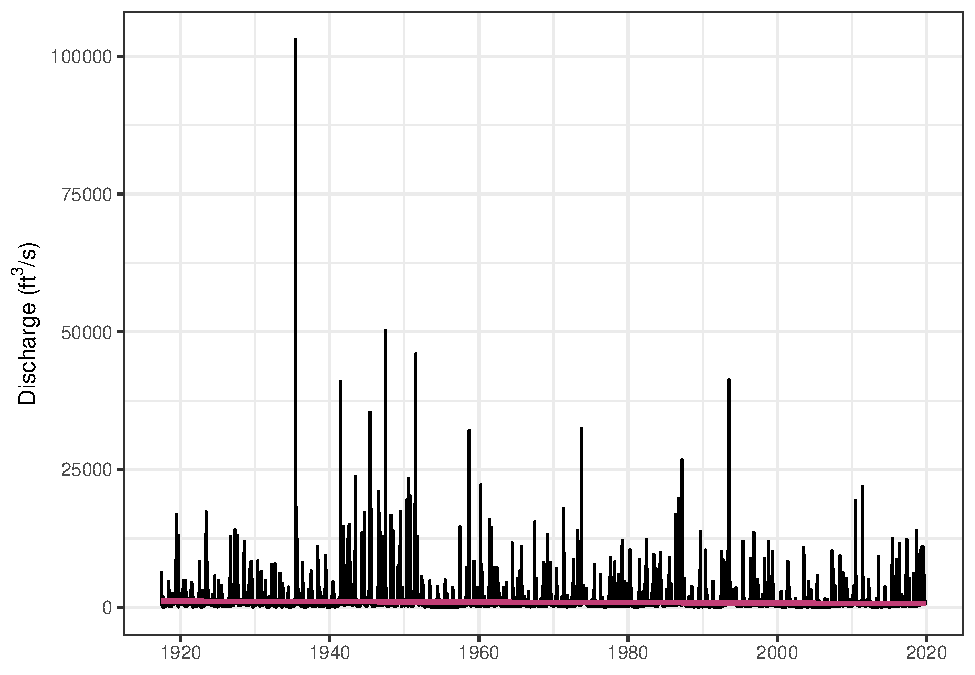
\includegraphics{Project_Template_files/figure-latex/unnamed-chunk-6-19.pdf}

\begin{Shaded}
\begin{Highlighting}[]
\NormalTok{RRCCDischarge <-}\StringTok{ }\KeywordTok{na.omit}\NormalTok{(RRCCDischarge)}
\NormalTok{RRCC_ts <-}\StringTok{ }\KeywordTok{ts}\NormalTok{(RRCCDischarge[[}\DecValTok{4}\NormalTok{]], }\DataTypeTok{frequency =} \DecValTok{365}\NormalTok{)}
\KeywordTok{table}\NormalTok{(}\KeywordTok{diff}\NormalTok{(RRCCDischarge}\OperatorTok{$}\NormalTok{Date))}
\end{Highlighting}
\end{Shaded}

\begin{verbatim}
## 
##     1 
## 37419
\end{verbatim}

\begin{Shaded}
\begin{Highlighting}[]
\CommentTok{# Generate the decomposition}
\NormalTok{RRCC_Decomposed <-}\StringTok{ }\KeywordTok{stl}\NormalTok{(RRCC_ts, }\DataTypeTok{s.window =} \StringTok{"periodic"}\NormalTok{)}

\CommentTok{# Visualize the decomposed series. }
\KeywordTok{plot}\NormalTok{(RRCC_Decomposed)}
\end{Highlighting}
\end{Shaded}

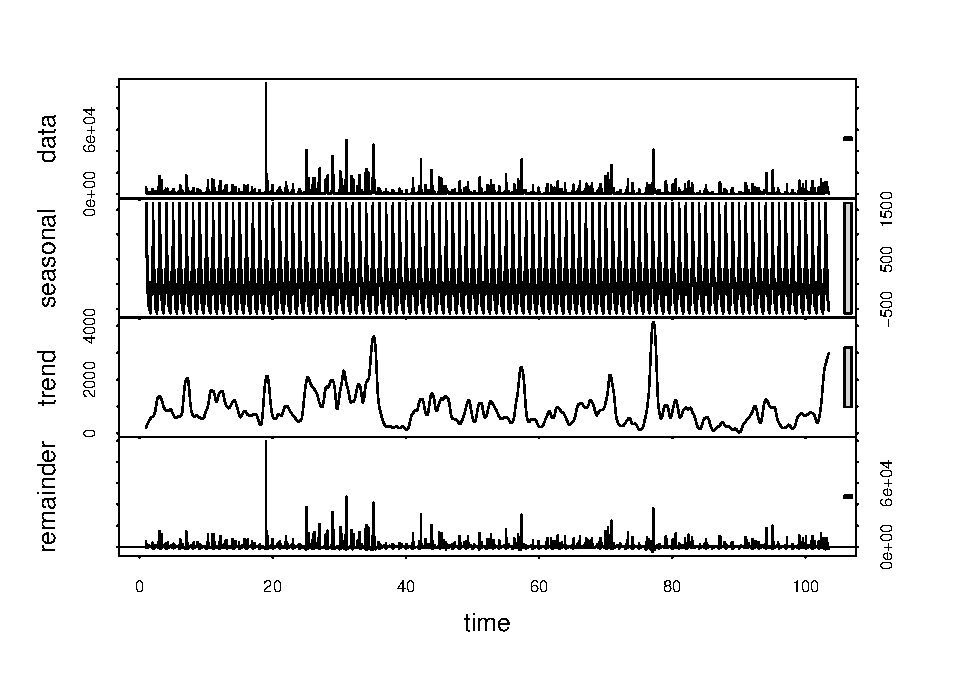
\includegraphics{Project_Template_files/figure-latex/unnamed-chunk-6-20.pdf}

\begin{Shaded}
\begin{Highlighting}[]
\CommentTok{# We can extract the components and turn them into data frames}
\NormalTok{RRCC_Components <-}\StringTok{ }\KeywordTok{as.data.frame}\NormalTok{(RRCC_Decomposed}\OperatorTok{$}\NormalTok{time.series[,}\DecValTok{1}\OperatorTok{:}\DecValTok{3}\NormalTok{])}
\NormalTok{RRCC_Components <-}\StringTok{ }\KeywordTok{mutate}\NormalTok{(RRCC_Components,}
                         \DataTypeTok{Observed =}\NormalTok{ RRCCDischarge}\OperatorTok{$}\NormalTok{Discharge,     }
                         \DataTypeTok{Date =}\NormalTok{ RRCCDischarge}\OperatorTok{$}\NormalTok{Date)}

\CommentTok{# Visualize how the trend maps onto the data}
\KeywordTok{ggplot}\NormalTok{(RRCC_Components) }\OperatorTok{+}
\StringTok{  }\KeywordTok{geom_line}\NormalTok{(}\KeywordTok{aes}\NormalTok{(}\DataTypeTok{y =}\NormalTok{ Observed, }\DataTypeTok{x =}\NormalTok{ Date),  }\DataTypeTok{size =} \FloatTok{0.25}\NormalTok{) }\OperatorTok{+}
\StringTok{  }\KeywordTok{geom_line}\NormalTok{(}\KeywordTok{aes}\NormalTok{(}\DataTypeTok{y =}\NormalTok{ trend, }\DataTypeTok{x =}\NormalTok{ Date), }\DataTypeTok{color =} \StringTok{"#c13d75ff"}\NormalTok{) }\OperatorTok{+}
\StringTok{  }\KeywordTok{geom_hline}\NormalTok{(}\DataTypeTok{yintercept =} \DecValTok{0}\NormalTok{, }\DataTypeTok{lty =} \DecValTok{2}\NormalTok{) }\OperatorTok{+}
\StringTok{  }\KeywordTok{ylab}\NormalTok{(}\KeywordTok{expression}\NormalTok{(}\StringTok{"Discharge (ft"}\OperatorTok{^}\DecValTok{3}\OperatorTok{*}\StringTok{"/s)"}\NormalTok{))}
\end{Highlighting}
\end{Shaded}

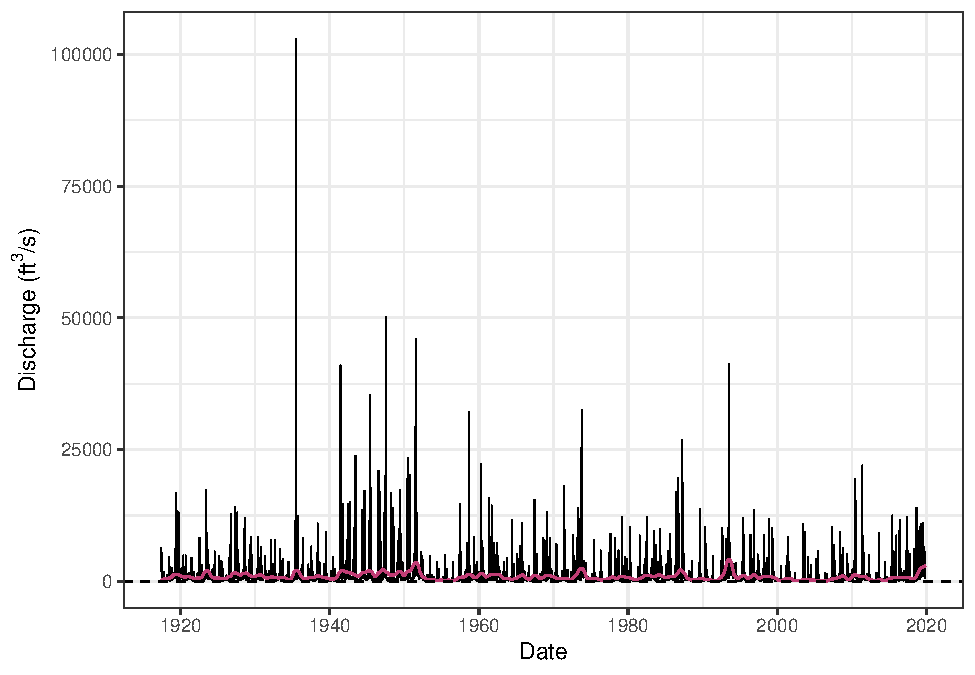
\includegraphics{Project_Template_files/figure-latex/unnamed-chunk-6-21.pdf}

\begin{Shaded}
\begin{Highlighting}[]
\CommentTok{# Visualize how the seasonal cycle maps onto the data}
\KeywordTok{ggplot}\NormalTok{(RRCC_Components) }\OperatorTok{+}
\StringTok{  }\KeywordTok{geom_line}\NormalTok{(}\KeywordTok{aes}\NormalTok{(}\DataTypeTok{y =}\NormalTok{ Observed, }\DataTypeTok{x =}\NormalTok{ Date),  }\DataTypeTok{size =} \FloatTok{0.25}\NormalTok{) }\OperatorTok{+}
\StringTok{  }\KeywordTok{geom_line}\NormalTok{(}\KeywordTok{aes}\NormalTok{(}\DataTypeTok{y =}\NormalTok{ seasonal, }\DataTypeTok{x =}\NormalTok{ Date), }\DataTypeTok{color =} \StringTok{"#c13d75ff"}\NormalTok{) }\OperatorTok{+}
\StringTok{  }\KeywordTok{geom_hline}\NormalTok{(}\DataTypeTok{yintercept =} \DecValTok{0}\NormalTok{, }\DataTypeTok{lty =} \DecValTok{2}\NormalTok{) }\OperatorTok{+}
\StringTok{  }\KeywordTok{ylab}\NormalTok{(}\KeywordTok{expression}\NormalTok{(}\StringTok{"Discharge (ft"}\OperatorTok{^}\DecValTok{3}\OperatorTok{*}\StringTok{"/s)"}\NormalTok{))}
\end{Highlighting}
\end{Shaded}

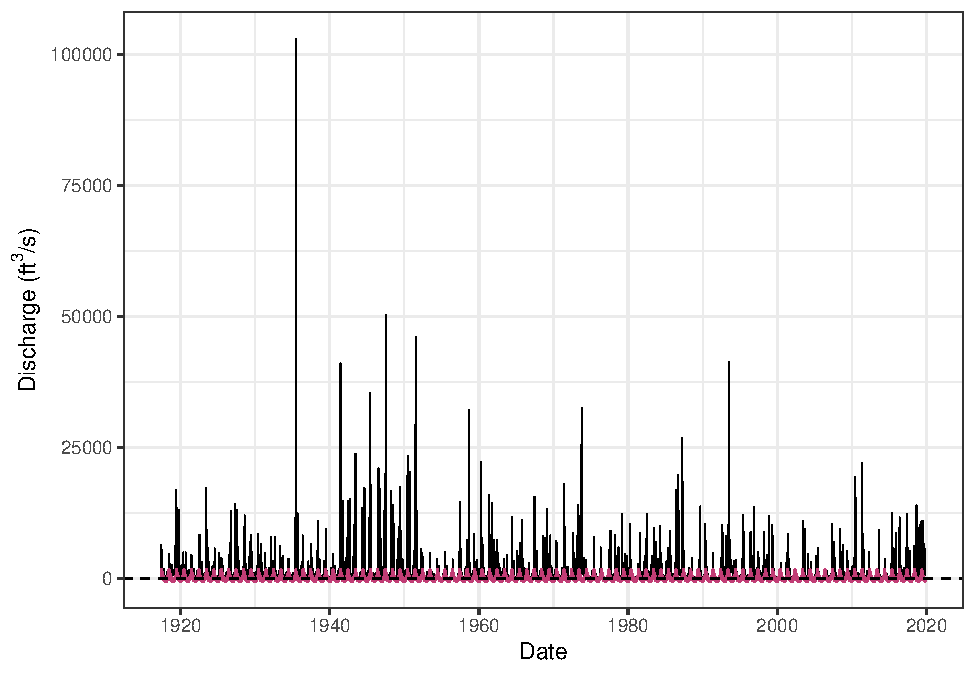
\includegraphics{Project_Template_files/figure-latex/unnamed-chunk-6-22.pdf}

\begin{Shaded}
\begin{Highlighting}[]
\NormalTok{RRCCDischarge.Monthly <-}\StringTok{ }\NormalTok{RRCCDischarge }\OperatorTok
\StringTok{  }\KeywordTok{mutate}\NormalTok{(}\DataTypeTok{Year =} \KeywordTok{year}\NormalTok{(Date),}
         \DataTypeTok{Month =} \KeywordTok{month}\NormalTok{(Date)) }\OperatorTok
\StringTok{  }\KeywordTok{group_by}\NormalTok{(Year, Month) }\OperatorTok
\StringTok{  }\KeywordTok{summarise}\NormalTok{(}\DataTypeTok{Discharge =} \KeywordTok{mean}\NormalTok{(Discharge))}
\NormalTok{RRCCMonthly_ts <-}\StringTok{ }\KeywordTok{ts}\NormalTok{(RRCCDischarge.Monthly[[}\DecValTok{3}\NormalTok{]], }\DataTypeTok{frequency =} \DecValTok{12}\NormalTok{)}
\KeywordTok{adf.test}\NormalTok{(RRCCMonthly_ts, }\DataTypeTok{alternative =} \StringTok{"stationary"}\NormalTok{)}
\end{Highlighting}
\end{Shaded}

\begin{verbatim}
## Warning in adf.test(RRCCMonthly_ts, alternative = "stationary"): p-value
## smaller than printed p-value
\end{verbatim}

\begin{verbatim}
## 
##  Augmented Dickey-Fuller Test
## 
## data:  RRCCMonthly_ts
## Dickey-Fuller = -7.4083, Lag order = 10, p-value = 0.01
## alternative hypothesis: stationary
\end{verbatim}

\begin{Shaded}
\begin{Highlighting}[]
\KeywordTok{acf}\NormalTok{(RRCCMonthly_ts)}
\end{Highlighting}
\end{Shaded}

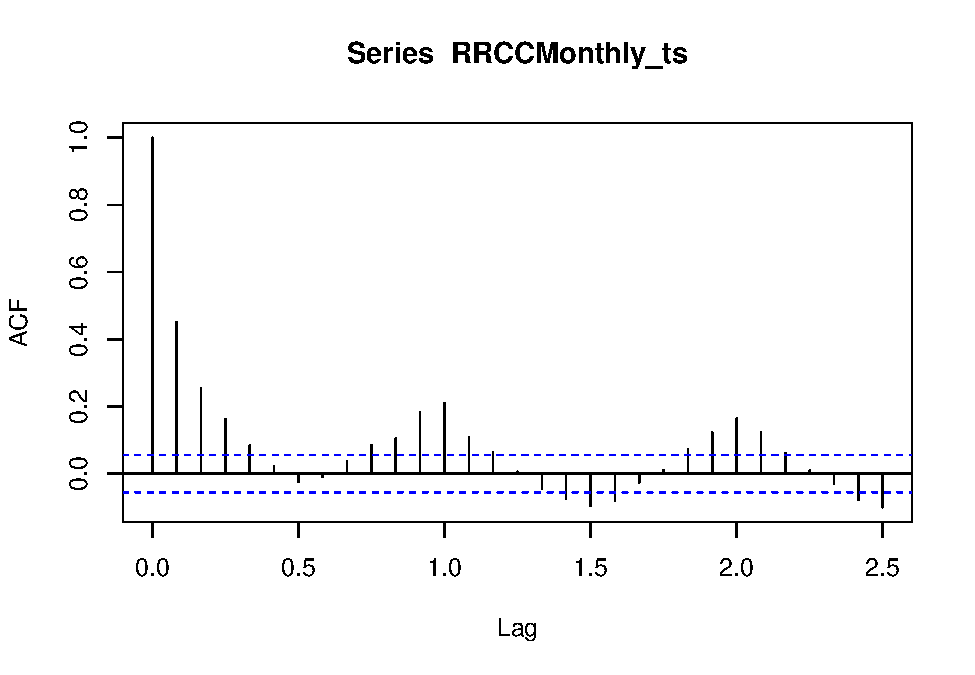
\includegraphics{Project_Template_files/figure-latex/unnamed-chunk-6-23.pdf}

\begin{Shaded}
\begin{Highlighting}[]
\KeywordTok{pacf}\NormalTok{(RRCCMonthly_ts)}
\end{Highlighting}
\end{Shaded}

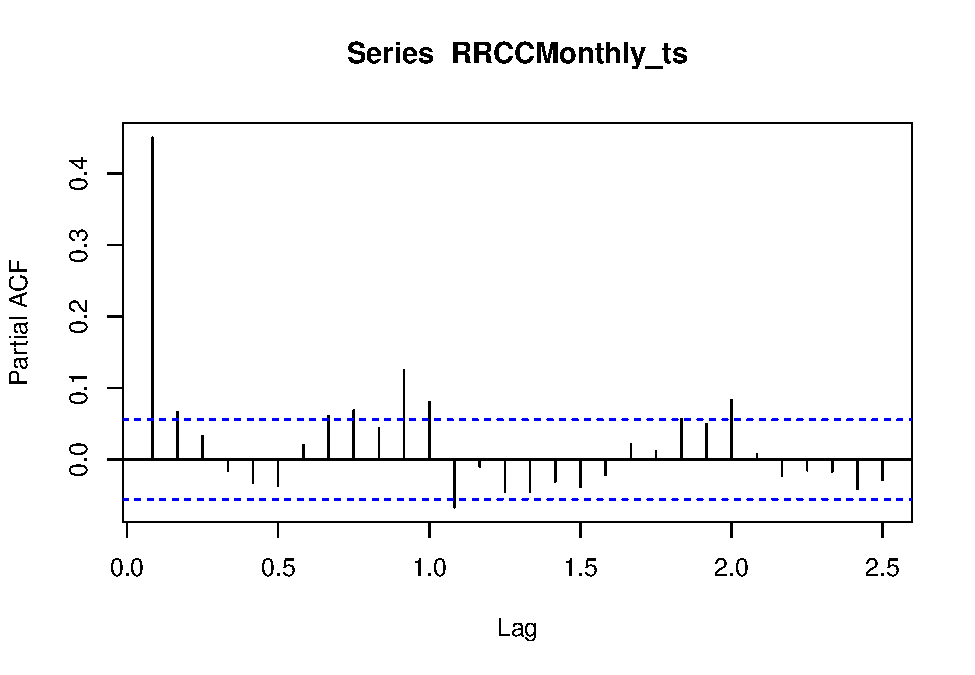
\includegraphics{Project_Template_files/figure-latex/unnamed-chunk-6-24.pdf}

\begin{Shaded}
\begin{Highlighting}[]
\CommentTok{# run the arima function and search for best fit}
\KeywordTok{auto.arima}\NormalTok{(RRCCMonthly_ts, }\DataTypeTok{trace =} \OtherTok{TRUE}\NormalTok{)}
\end{Highlighting}
\end{Shaded}

\begin{verbatim}
## 
##  Fitting models using approximations to speed things up...
## 
##  ARIMA(2,1,2)(1,0,1)[12] with drift         : Inf
##  ARIMA(0,1,0)            with drift         : 21233.6
##  ARIMA(1,1,0)(1,0,0)[12] with drift         : 21088.27
##  ARIMA(0,1,1)(0,0,1)[12] with drift         : 20969.16
##  ARIMA(0,1,0)                               : 21231.6
##  ARIMA(0,1,1)            with drift         : 20998.71
##  ARIMA(0,1,1)(1,0,1)[12] with drift         : Inf
##  ARIMA(0,1,1)(0,0,2)[12] with drift         : 20952.71
##  ARIMA(0,1,1)(1,0,2)[12] with drift         : Inf
##  ARIMA(0,1,0)(0,0,2)[12] with drift         : 21216.56
##  ARIMA(1,1,1)(0,0,2)[12] with drift         : 20830.75
##  ARIMA(1,1,1)(0,0,1)[12] with drift         : 20837.91
##  ARIMA(1,1,1)(1,0,2)[12] with drift         : Inf
##  ARIMA(1,1,1)(1,0,1)[12] with drift         : Inf
##  ARIMA(1,1,0)(0,0,2)[12] with drift         : 21073.73
##  ARIMA(2,1,1)(0,0,2)[12] with drift         : 20819.33
##  ARIMA(2,1,1)(0,0,1)[12] with drift         : 20827.19
##  ARIMA(2,1,1)(1,0,2)[12] with drift         : Inf
##  ARIMA(2,1,1)(1,0,1)[12] with drift         : Inf
##  ARIMA(2,1,0)(0,0,2)[12] with drift         : 21009.64
##  ARIMA(3,1,1)(0,0,2)[12] with drift         : 20819.54
##  ARIMA(2,1,2)(0,0,2)[12] with drift         : Inf
##  ARIMA(1,1,2)(0,0,2)[12] with drift         : 20832.46
##  ARIMA(3,1,0)(0,0,2)[12] with drift         : 20983.45
##  ARIMA(3,1,2)(0,0,2)[12] with drift         : 20822.26
##  ARIMA(2,1,1)(0,0,2)[12]                    : 20817.47
##  ARIMA(2,1,1)(0,0,1)[12]                    : 20825.33
##  ARIMA(2,1,1)(1,0,2)[12]                    : Inf
##  ARIMA(2,1,1)(1,0,1)[12]                    : Inf
##  ARIMA(1,1,1)(0,0,2)[12]                    : 20829.04
##  ARIMA(2,1,0)(0,0,2)[12]                    : 21007.62
##  ARIMA(3,1,1)(0,0,2)[12]                    : 20817.66
##  ARIMA(2,1,2)(0,0,2)[12]                    : Inf
##  ARIMA(1,1,0)(0,0,2)[12]                    : 21071.71
##  ARIMA(1,1,2)(0,0,2)[12]                    : 20830.76
##  ARIMA(3,1,0)(0,0,2)[12]                    : 20981.43
##  ARIMA(3,1,2)(0,0,2)[12]                    : 20820.4
## 
##  Now re-fitting the best model(s) without approximations...
## 
##  ARIMA(2,1,1)(0,0,2)[12]                    : Inf
##  ARIMA(3,1,1)(0,0,2)[12]                    : Inf
##  ARIMA(2,1,1)(0,0,2)[12] with drift         : Inf
##  ARIMA(3,1,1)(0,0,2)[12] with drift         : Inf
##  ARIMA(3,1,2)(0,0,2)[12]                    : Inf
##  ARIMA(3,1,2)(0,0,2)[12] with drift         : Inf
##  ARIMA(2,1,1)(0,0,1)[12]                    : Inf
##  ARIMA(2,1,1)(0,0,1)[12] with drift         : Inf
##  ARIMA(1,1,1)(0,0,2)[12]                    : Inf
##  ARIMA(1,1,1)(0,0,2)[12] with drift         : Inf
##  ARIMA(1,1,2)(0,0,2)[12]                    : Inf
##  ARIMA(1,1,2)(0,0,2)[12] with drift         : Inf
##  ARIMA(1,1,1)(0,0,1)[12] with drift         : Inf
##  ARIMA(0,1,1)(0,0,2)[12] with drift         : 20966.7
## 
##  Best model: ARIMA(0,1,1)(0,0,2)[12] with drift
\end{verbatim}

\begin{verbatim}
## Series: RRCCMonthly_ts 
## ARIMA(0,1,1)(0,0,2)[12] with drift 
## 
## Coefficients:
##           ma1    sma1    sma2    drift
##       -0.6719  0.1524  0.1086   1.4116
## s.e.   0.0403  0.0288  0.0252  14.3820
## 
## sigma^2 estimated as 1492963:  log likelihood=-10478.33
## AIC=20966.66   AICc=20966.7   BIC=20992.23
\end{verbatim}

\begin{Shaded}
\begin{Highlighting}[]
\CommentTok{# create an object that defines the best fit model}
\NormalTok{RRCCfit <-}\StringTok{ }\KeywordTok{arima}\NormalTok{(RRCCMonthly_ts, }\KeywordTok{c}\NormalTok{(}\DecValTok{0}\NormalTok{, }\DecValTok{1}\NormalTok{, }\DecValTok{1}\NormalTok{),}\DataTypeTok{seasonal =} \KeywordTok{list}\NormalTok{(}\DataTypeTok{order =} \KeywordTok{c}\NormalTok{(}\DecValTok{0}\NormalTok{, }\DecValTok{0}\NormalTok{, }\DecValTok{2}\NormalTok{), }\DataTypeTok{period =} \DecValTok{12}\NormalTok{))}

\CommentTok{# make a prediction into the future}
\NormalTok{RRCCprediction <-}\StringTok{ }\KeywordTok{predict}\NormalTok{(RRCCfit, }\DataTypeTok{n.ahead =} \DecValTok{10}\OperatorTok{*}\DecValTok{12}\NormalTok{)}

\CommentTok{# plot future predictions}
\KeywordTok{ts.plot}\NormalTok{(RRCCMonthly_ts, RRCCprediction}\OperatorTok{$}\NormalTok{pred, }\DataTypeTok{lty =} \KeywordTok{c}\NormalTok{(}\DecValTok{1}\NormalTok{, }\DecValTok{3}\NormalTok{))}
\end{Highlighting}
\end{Shaded}

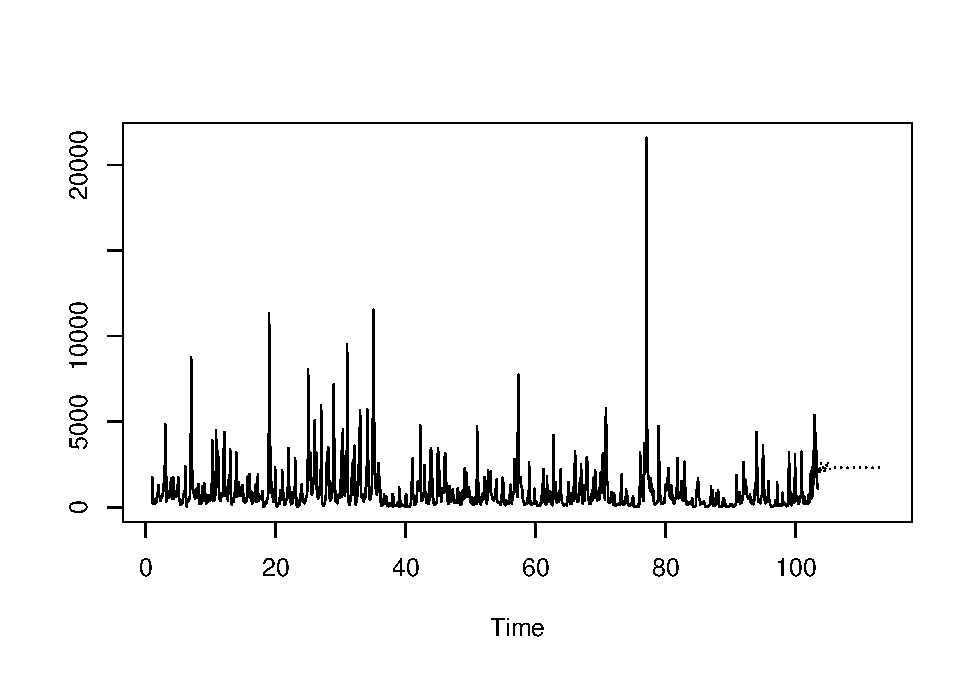
\includegraphics{Project_Template_files/figure-latex/unnamed-chunk-6-25.pdf}

\begin{Shaded}
\begin{Highlighting}[]
\CommentTok{########################### Nitrogen Analysis ############################}
\CommentTok{# Generate monthly values from February 1973 to September 1993}
\NormalTok{RRCCNitrogenlp <-}\StringTok{ }\KeywordTok{as.data.frame}\NormalTok{(}\KeywordTok{approx}\NormalTok{(RRCCNitrogen, }\DataTypeTok{n =} \DecValTok{249}\NormalTok{, }\DataTypeTok{method =} \StringTok{"linear"}\NormalTok{))}
\NormalTok{RRCCNitrogenlp}\OperatorTok{$}\NormalTok{x <-}\StringTok{ }\KeywordTok{as.Date}\NormalTok{(RRCCNitrogenlp}\OperatorTok{$}\NormalTok{x, }\DataTypeTok{origin =} \StringTok{"1970-01-01"}\NormalTok{)}
\KeywordTok{names}\NormalTok{(RRCCNitrogenlp) <-}\StringTok{ }\KeywordTok{c}\NormalTok{(}\StringTok{"Date"}\NormalTok{, }\StringTok{"N"}\NormalTok{)}

\CommentTok{# Inspect interpolated values}
\NormalTok{RRCCNinterpolated <-}
\StringTok{  }\KeywordTok{ggplot}\NormalTok{(RRCCNitrogen, }\KeywordTok{aes}\NormalTok{(}\DataTypeTok{x =}\NormalTok{ sample_dt, }\DataTypeTok{y =}\NormalTok{ result_va)) }\OperatorTok{+}
\StringTok{  }\KeywordTok{geom_point}\NormalTok{() }\OperatorTok{+}
\StringTok{  }\KeywordTok{geom_line}\NormalTok{() }\OperatorTok{+}
\StringTok{  }\KeywordTok{geom_point}\NormalTok{(}\DataTypeTok{data =}\NormalTok{ RRCCNitrogenlp, }\KeywordTok{aes}\NormalTok{(}\DataTypeTok{x =}\NormalTok{ Date, }\DataTypeTok{y =}\NormalTok{ N), }\DataTypeTok{color =} \StringTok{"#c13d75ff"}\NormalTok{)}
\KeywordTok{print}\NormalTok{(RRCCNinterpolated)}
\end{Highlighting}
\end{Shaded}

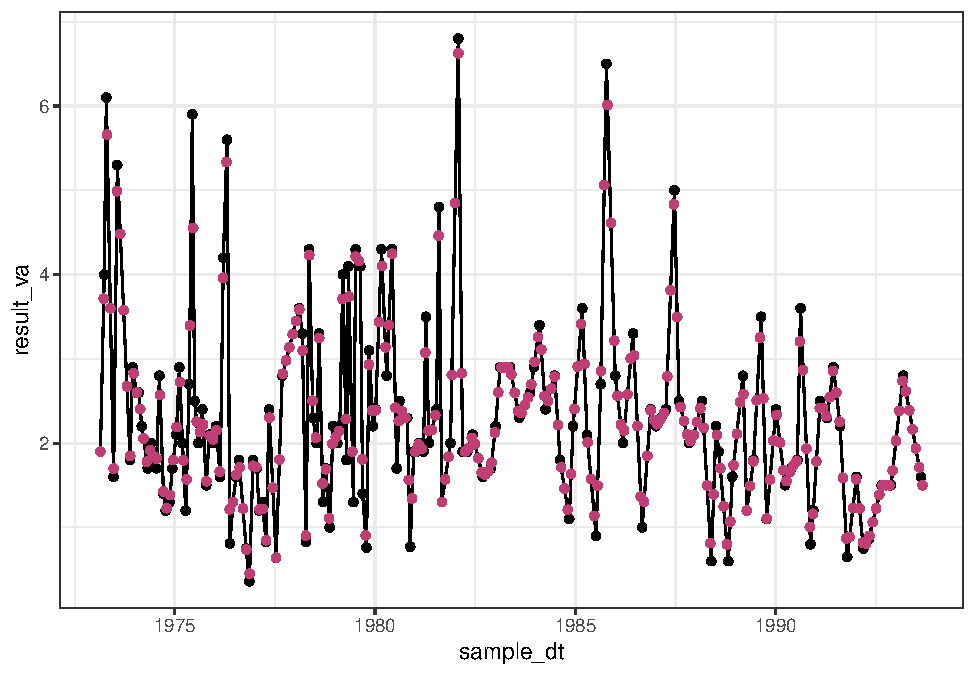
\includegraphics{Project_Template_files/figure-latex/unnamed-chunk-6-26.pdf}

\begin{Shaded}
\begin{Highlighting}[]
\CommentTok{# Generate time series (smk.test needs ts, not data.frame)}
\NormalTok{RRCCNtimeseries <-}\StringTok{ }\KeywordTok{ts}\NormalTok{(RRCCNitrogenlp}\OperatorTok{$}\NormalTok{N, }\DataTypeTok{frequency =} \DecValTok{12}\NormalTok{,}
                     \DataTypeTok{start =} \KeywordTok{c}\NormalTok{(}\DecValTok{1973}\NormalTok{, }\DecValTok{2}\NormalTok{, }\DecValTok{22}\NormalTok{), }\DataTypeTok{end =} \KeywordTok{c}\NormalTok{(}\DecValTok{1993}\NormalTok{, }\DecValTok{9}\NormalTok{, }\DecValTok{1}\NormalTok{))}
\CommentTok{# Run SMK test}
\NormalTok{RRCCNtrend <-}\StringTok{ }\KeywordTok{smk.test}\NormalTok{(RRCCNtimeseries)}

\CommentTok{# Inspect results}
\NormalTok{RRCCNtrend}
\end{Highlighting}
\end{Shaded}

\begin{verbatim}
## 
##  Seasonal Mann-Kendall trend test (Hirsch-Slack test)
## 
## data:  RRCCNtimeseries
## z = -3.0233, p-value = 0.002501
## alternative hypothesis: true S is not equal to 0
## sample estimates:
##        S     varS 
##  -340.00 12573.33
\end{verbatim}

\begin{Shaded}
\begin{Highlighting}[]
\KeywordTok{summary}\NormalTok{(RRCCNtrend)}
\end{Highlighting}
\end{Shaded}

\begin{verbatim}
## 
##  Seasonal Mann-Kendall trend test (Hirsch-Slack test)
## 
## data: RRCCNtimeseries
## alternative hypothesis: two.sided
## 
## Statistics for individual seasons
## 
## H0
##                      S   varS    tau      z Pr(>|z|)  
## Season 1:   S = 0  -66  950.0 -0.347 -2.109 0.034955 *
## Season 2:   S = 0  -32 1096.7 -0.152 -0.936 0.349219  
## Season 3:   S = 0  -40 1096.7 -0.190 -1.178 0.238924  
## Season 4:   S = 0  -18 1096.7 -0.086 -0.513 0.607708  
## Season 5:   S = 0  -60 1096.7 -0.286 -1.782 0.074811 .
## Season 6:   S = 0   -6 1096.7 -0.029 -0.151 0.879988  
## Season 7:   S = 0  -12 1096.7 -0.057 -0.332 0.739764  
## Season 8:   S = 0  -46 1096.7 -0.219 -1.359 0.174190  
## Season 9:   S = 0   16 1096.7  0.076  0.453 0.650582  
## Season 10:   S = 0  16  950.0  0.084  0.487 0.626496  
## Season 11:   S = 0 -20  950.0 -0.105 -0.616 0.537603  
## Season 12:   S = 0 -72  950.0 -0.379 -2.304 0.021248 *
## ---
## Signif. codes:  0 '***' 0.001 '**' 0.01 '*' 0.05 '.' 0.1 ' ' 1
\end{verbatim}

\begin{Shaded}
\begin{Highlighting}[]
\CommentTok{########################### Phosphorus Analysis ############################}
\CommentTok{# Generate monthly values from January 1973 to September 1993}
\NormalTok{RRCCPhosphoruslp <-}\StringTok{ }\KeywordTok{as.data.frame}\NormalTok{(}\KeywordTok{approx}\NormalTok{(RRCCPhosphorus, }\DataTypeTok{n =} \DecValTok{250}\NormalTok{, }\DataTypeTok{method =} \StringTok{"linear"}\NormalTok{))}
\NormalTok{RRCCPhosphoruslp}\OperatorTok{$}\NormalTok{x <-}\StringTok{ }\KeywordTok{as.Date}\NormalTok{(RRCCPhosphoruslp}\OperatorTok{$}\NormalTok{x, }\DataTypeTok{origin =} \StringTok{"1970-01-01"}\NormalTok{)}
\KeywordTok{names}\NormalTok{(RRCCPhosphoruslp) <-}\StringTok{ }\KeywordTok{c}\NormalTok{(}\StringTok{"Date"}\NormalTok{, }\StringTok{"P"}\NormalTok{)}

\CommentTok{# Inspect interpolated values}
\NormalTok{RRCCPinterpolated <-}
\StringTok{  }\KeywordTok{ggplot}\NormalTok{(RRCCPhosphorus, }\KeywordTok{aes}\NormalTok{(}\DataTypeTok{x =}\NormalTok{ sample_dt, }\DataTypeTok{y =}\NormalTok{ result_va)) }\OperatorTok{+}
\StringTok{  }\KeywordTok{geom_point}\NormalTok{() }\OperatorTok{+}
\StringTok{  }\KeywordTok{geom_line}\NormalTok{() }\OperatorTok{+}
\StringTok{  }\KeywordTok{geom_point}\NormalTok{(}\DataTypeTok{data =}\NormalTok{ RRCCPhosphoruslp, }\KeywordTok{aes}\NormalTok{(}\DataTypeTok{x =}\NormalTok{ Date, }\DataTypeTok{y =}\NormalTok{ P), }\DataTypeTok{color =} \StringTok{"#c13d75ff"}\NormalTok{)}
\KeywordTok{print}\NormalTok{(RRCCPinterpolated)}
\end{Highlighting}
\end{Shaded}

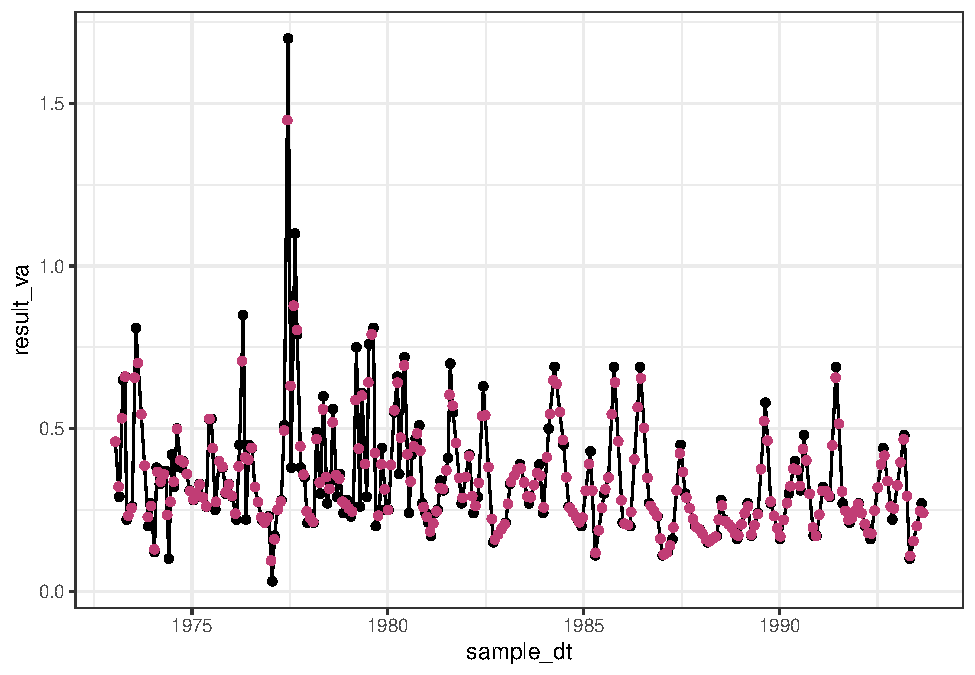
\includegraphics{Project_Template_files/figure-latex/unnamed-chunk-6-27.pdf}

\begin{Shaded}
\begin{Highlighting}[]
\CommentTok{# Generate time series (smk.test needs ts, not data.frame)}
\NormalTok{RRCCPtimeseries <-}\StringTok{ }\KeywordTok{ts}\NormalTok{(RRCCPhosphoruslp}\OperatorTok{$}\NormalTok{P, }\DataTypeTok{frequency =} \DecValTok{12}\NormalTok{,}
                     \DataTypeTok{start =} \KeywordTok{c}\NormalTok{(}\DecValTok{1973}\NormalTok{, }\DecValTok{1}\NormalTok{, }\DecValTok{16}\NormalTok{), }\DataTypeTok{end =} \KeywordTok{c}\NormalTok{(}\DecValTok{1993}\NormalTok{, }\DecValTok{9}\NormalTok{, }\DecValTok{1}\NormalTok{))}
\CommentTok{# Run SMK test}
\NormalTok{RRCCPtrend <-}\StringTok{ }\KeywordTok{smk.test}\NormalTok{(RRCCPtimeseries)}

\CommentTok{# Inspect results}
\NormalTok{RRCCPtrend}
\end{Highlighting}
\end{Shaded}

\begin{verbatim}
## 
##  Seasonal Mann-Kendall trend test (Hirsch-Slack test)
## 
## data:  RRCCPtimeseries
## z = -4.7614, p-value = 1.923e-06
## alternative hypothesis: true S is not equal to 0
## sample estimates:
##     S  varS 
##  -538 12720
\end{verbatim}

\begin{Shaded}
\begin{Highlighting}[]
\KeywordTok{summary}\NormalTok{(RRCCPtrend)}
\end{Highlighting}
\end{Shaded}

\begin{verbatim}
## 
##  Seasonal Mann-Kendall trend test (Hirsch-Slack test)
## 
## data: RRCCPtimeseries
## alternative hypothesis: two.sided
## 
## Statistics for individual seasons
## 
## H0
##                      S   varS    tau      z Pr(>|z|)  
## Season 1:   S = 0  -42 1096.7 -0.200 -1.238 0.215689  
## Season 2:   S = 0  -32 1096.7 -0.152 -0.936 0.349219  
## Season 3:   S = 0  -54 1096.7 -0.257 -1.600 0.109502  
## Season 4:   S = 0  -68 1096.7 -0.324 -2.023 0.043053 *
## Season 5:   S = 0  -40 1096.7 -0.190 -1.178 0.238924  
## Season 6:   S = 0  -52 1096.7 -0.248 -1.540 0.123550  
## Season 7:   S = 0  -60 1096.7 -0.286 -1.782 0.074811 .
## Season 8:   S = 0  -62 1096.7 -0.295 -1.842 0.065473 .
## Season 9:   S = 0  -54 1096.7 -0.257 -1.600 0.109502  
## Season 10:   S = 0  -4  950.0 -0.021 -0.097 0.922462  
## Season 11:   S = 0 -20  950.0 -0.105 -0.616 0.537603  
## Season 12:   S = 0 -50  950.0 -0.263 -1.590 0.111887  
## ---
## Signif. codes:  0 '***' 0.001 '**' 0.01 '*' 0.05 '.' 0.1 ' ' 1
\end{verbatim}

\newpage

\hypertarget{summary-and-conclusions}{%
\section{Summary and Conclusions}\label{summary-and-conclusions}}

\textless{}Summarize your major findings from your analyses. What
conclusions do you draw from your findings? Make sure to apply this to a
broader application for the research question you have
answered.\textgreater{}

\hypertarget{example-for-autoreferencing}{%
\subsection{Example for
autoreferencing}\label{example-for-autoreferencing}}

As seen by \autoref{fig:foo}, Absorbance values are not normally
distributed. This is expected, as we are dealing with ecological data.

\begin{figure}
\centering
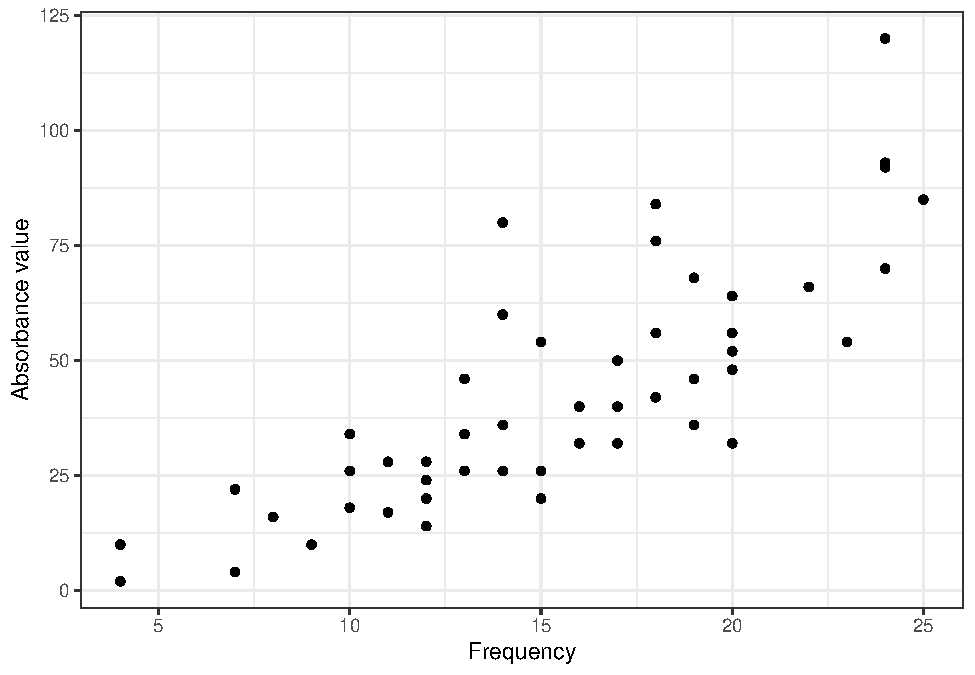
\includegraphics{Project_Template_files/figure-latex/foo-1.pdf}
\caption{\label{fig:foo}Absorbance frequency}
\end{figure}


\end{document}
